\chapter{Experimental Setup}
\label{chap:Detector}
%\cite{Evans:2008zzb} \cite{LEP}
The hadron colliders aim at search for elementary particles and their interactions as predicted in the Standard Model or theories beyond the Standard Model. For the same beam energy, higher center-of-mass energy can be achieved by the hadron colliders as compared to fixed target experiments. Due to the availability of very high center-of-mass energy for the collisions, it becomes possible for the researchers to understand the fundamental structure of the universe deeply and to look back in its history. The precise measurement of mass of the $Z$ and $W$ boson discovered by the UA1 and UA2 experiments was done at the Large Electron-Positron (LEP) collider. The discovery of top quark and an acute measurement of its mass was performed by the proton-antiproton collider Tevatron at FNAL. The search for the long awaited Higgs boson was carried out by the currently running most powerful accelerator, the Large Hadron Collider (LHC). Still many questions related to the the nature of dark matter, the existence of super-symmetry (SUSY) or the extra dimensions are yet to be answered. 

The European Organization for Nuclear Research (CERN) is a world-class fundamental physics research organization founded in 1954. In the beginning, it concentrated on pure physics research to understand the inside of the atom, justifying the word ``nuclear'' in name. At present, the main area of research at CERN is particle physics - the study of the fundamental constituents of matter and the forces of interactions acting between them. To complete this task, several particle accelerators have been built by CERN to explore the physics at the TeV energy scale.

\section{The Large Hadron Collider}
The Large Hadron Collider (LHC) \cite{Evans:2008zzb} is the world's biggest and the most powerful particle accelerator and collider built by CERN. It occupies the 27 km circumference circular tunnel (between the border of France and Switzerland), previously used by LEP collider \cite{LEP}, at a depth ranging from 50 to 175 metres (164 to 574 ft) underground. Two beams of particles of the same kind, either protons or lead or xenon ions, are accelerated in direction opposite to each other. 1,232 dipole magnets maintain the beams in their circular path and 392 quadrupole magnets keep the beams focused to increase the probabilities of interaction between the particles. Since this thesis is based on the proton-proton (pp) collisions data, the main focus is on protons. 

The protons pass through a series of accelerators which increase their energy successively before their injection into the main ring of LHC. Figure~\ref{fig:LHC} gives an overview of the various accelerators and detectors comprising the complex structure of the LHC. The protons are obtained by stripping of electrons from hydrogen gas atoms using an electric field. The protons are accelerated up to 100 keV through a radiofrequency quadrupole which provides the first focusing and a further acceleration to 750 keV energy. The linear particle accelerator (LINAC2) increases the energy of protons to 50 MeV. Then these protons are injected into the Proton Synchrotron Booster (PSB) in the form of bunches where they get accelerated to 1.4 GeV energy. The energy of protons is further enhanced to 25 GeV by Proton Synchrotron (PS) and then to 450 GeV by the Super Proton Synchrotron (SPS). Finally the protons are injected into two beam pipelines of the main LHC ring where their energy increases to the collision energy. In head on collisions for colliding beams of the same mass particles, the center of mass system and the laboratory system coincide and the total center of mass energy is twice the energy of the beams. 

\begin{figure}[!h]
 \begin{center} 
 \hspace*{-5mm}
 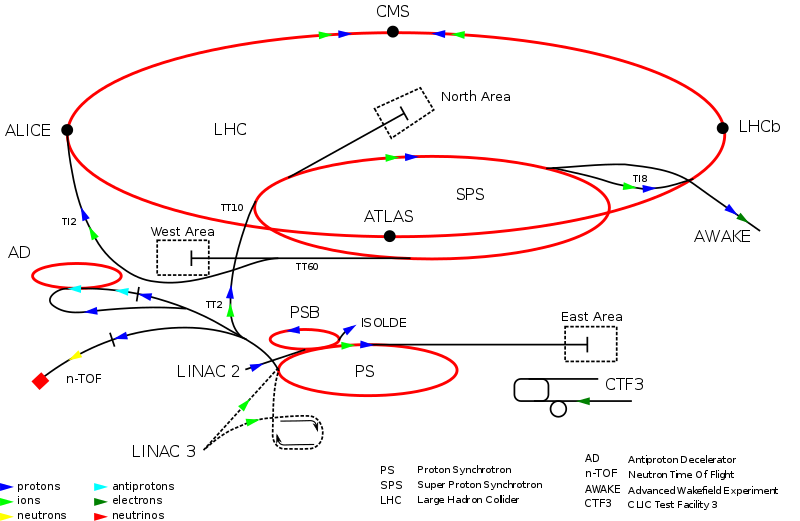
\includegraphics[width=1.\textwidth]{/home/anter/Desktop/Thesis/Figures/LHC.png}\\
 \vspace*{5mm}
 \caption[Overview of the different experiments of the Large Hadron Collider (LHC), a complex particle accelerator and collider located at CERN.]{Overview of the different experiments of the Large Hadron Collider (LHC), a complex particle accelerator and collider located at CERN\footnotemark.}
 \label{fig:LHC}
 \end{center}
\end{figure}
\footnotetext{Source : \url{https://en.wikipedia.org/wiki/Large_Hadron_Collider}}

The accelerated beams are made to collide at four interaction points around which six detectors : ALICE (A Large Ion Collider Experiment) \cite{Aamodt:2008zz}, ATLAS (A Toroidal LHC Apparatus) \cite{Aad:2008zzm}, CMS (Compact Muon Solenoid) \cite{Chatrchyan:2008aa,Bayatian:2006nff,Ball:2007zza}, LHCb (Large Hadron Collider for Beauty) \cite{Alves:2008zz}, LHCf (Large Hadron Collider forward)\cite{Adriani:2008zz} and TOTEM (Total, elastic and diffractive cross-section measurement) \cite{Anelli:2008zza}, are located. The CMS and ATLAS are the two general purpose detectors dedicated to the search of the Higgs boson, existence of super-symmetry (SUSY) and also looking for extra dimensions. The ALICE is a heavy-ion detector which collides lead ions to study quark-gluon plasma, a state of matter believed to be present just after the Big Bang. The LHCb experiment will explore the differences between matter and antimatter and new physics through b-quark (beauty) studies. TOTEM experiment is dedicated to cross-section measurements whereas LHCf focuses on forward physics. 

The LHC successfully injected the first protons on September 10, 2008 but after few days magnetic quench occurred in about 100 bending magnets leading to a loss of $\sim$6 tonnes of liquid helium. The low-energy beams circulated in the tunnel for the first time on November 20, 2009 and after three days, the first particle collisions took place in all four detectors at \cme = 450 GeV. The LHC achieved 1.18 TeV energy per beam on November 30, 2009 and become the world’s highest energy particle accelerator leaving behind the Tevatron with record of 0.98 TeV per beam for eight years. The pp collisions at \cme = 2.36 TeV were recorded around December 15, 2009. On March 19, 2010, the beam energy was ramped up to 3.5 TeV, resulting in the first pp collisions at \cme = 7 TeV on March 30, 2010. The beam energy was kept at 3.5 TeV throughout 2011, and increased to 4 TeV in 2012. After a long shutdown for two years, the LHC restarted in 2015 and collided the proton beams at a much higher centre-of-mass energy of 13 TeV and is running successfully till now. In the coming years, protons will be made to collide at a designed \cme = 14 TeV with luminosity up to 10$^{34}$ cm$^{-2}$s$^{-1}$. In this thesis, work has been carried out using the pp collisions data collected by the CMS detector at \cme = 8 TeV in the year of 2012.

\subsection{Luminosity Measurement}
\label{sec:lumi}
Luminosity (\lumi) is one of the most important parameters of an accelerator which characterizes its performance. It gives the rate at which collisions occur and given by the number of collisions produced in a detector per cm$^2$ and per second. Cross-section ($\sigma$) is a measurement of the probability that an event will occur. It is related to total number of events $N$ of a process over a time period T and \lumi as :
\begin{equation}
N = \int_{0}^{T} \lumi~\sigma~dt = \lumi_{int}~\sigma
\end{equation}
where $\int_{0}^{T} \lumi~dt = \lumi_{int}$ is the total integrated luminosity. It is expressed in units of area, usually in barn$^{-1}$ and gives a direct indication of the number of produced events for a process. For example, an integrated luminosity of 10 fb$^{-1}$ means that 10 events are produced in a process with cross-section equal to 1 fb.

The luminosity depends on the particle beam parameters and is given by :

\begin{equation}
\lumi = \frac{N^2_p~N_b~f_{rev}~\gamma~F}{4\pi~\epsilon_n~\beta^*}
\end{equation}
where $N_p$ is the number of particles per bunch, $N_b$ is the number of bunches per beam, $f_{rev}$ is the revolution frequency of the beam, $\gamma$ is the relativistic gamma factor and $F$ gives the geometric luminosity reduction factor. The effective collision area of the two beams is related to the normalized transverse beam emittance $\epsilon_n$ and the value of the betatron function $ \beta^*$ at the interaction point.
 
The CMS experiment constantly monitors the instantaneous luminosity delivered by LHC which is shown versus time in Fig.~\ref{fig:lumi} for proton-proton collisions at nominal center-of-mass energy for the years 2010-2017. The relative instantaneous luminosity is calculated by using two methods \cite{CMS:2013gfa} : Hadron Forward (HF) method by measuring the particle flux in the hadron forward calorimeter and by counting the number of reconstructed vertices in the pixel tracker. The absolute luminosity measurement relies on van-der-Meer scans done in special runs of the LHC \cite{vanderMeer:1968zz}. The uncertainty on the luminosity measured for 2012 data set is 2.5\% (syst.) and 0.5\% (stat.).

\begin{figure}[!h]
 \begin{center}
 \vspace*{4mm} 
 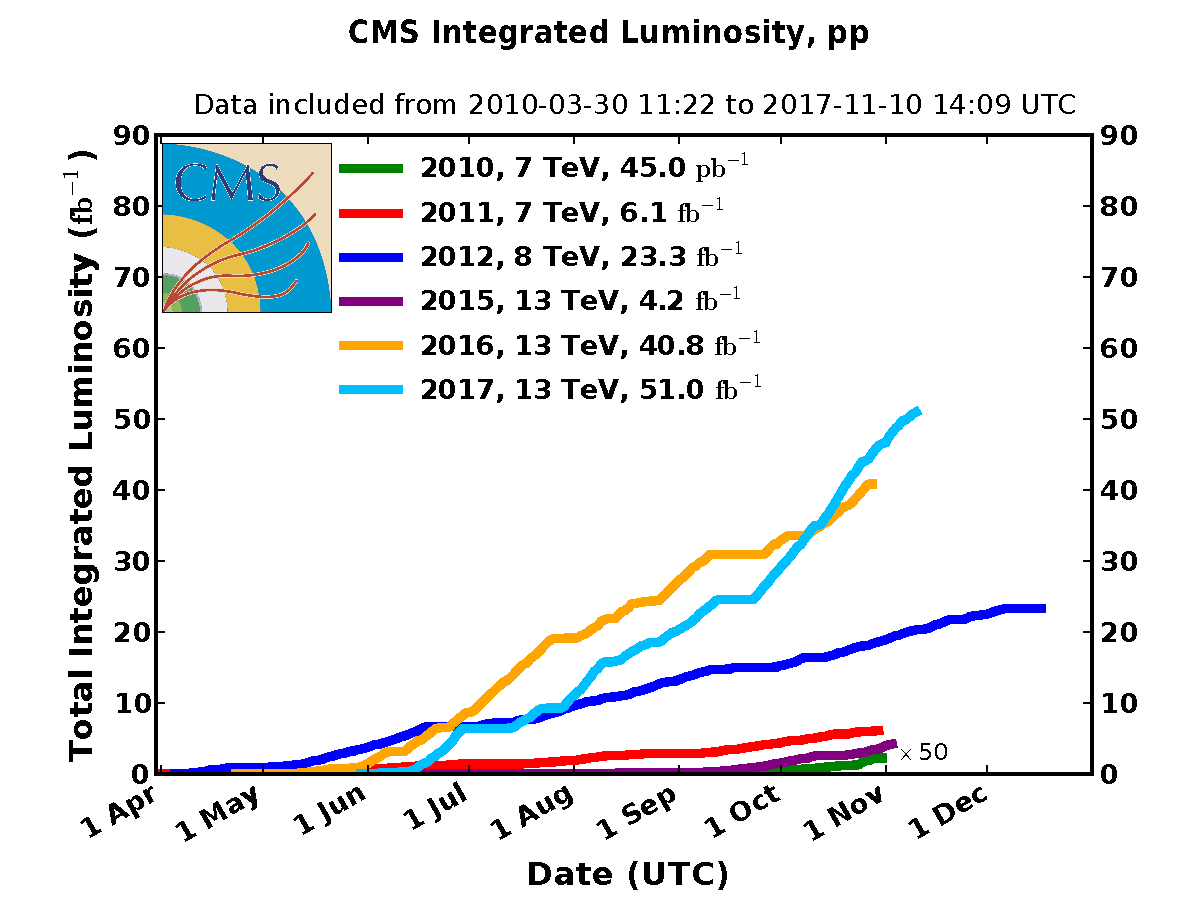
\includegraphics[width=.8\textwidth]{/home/anter/Desktop/Thesis/Figures/int_lumi_cumulative_pp_2.pdf}\\
 \vspace*{5mm}
 \caption[The integrated luminosity, delivered to CMS during stable beams for proton-proton collisions.]{The integrated luminosity, delivered to CMS during stable beams for proton-proton collisions at nominal center-of-mass energy, is shown versus time for data-taking in 2010 (green), 2011 (red), 2012 (blue), 2015 (purple), 2016 (orange) and 2017 (light blue) run periods of the LHC\footnotemark.}
 \label{fig:lumi}
 \end{center}
\end{figure}
\footnotetext{Source : \url{https://twiki.cern.ch/twiki/bin/view/CMSPublic/LumiPublicResults}}

\subsection{Pileup Interactions}
To observe the extremely rare events, the event rate in a collider should be very high. This demands delivered luminosity to be high which is achieved by increasing the number of bunches or increasing the number of protons per bunch. However, this comes at the cost of multiple proton-proton interactions coming from independent hadron-hadron collisions occurring in the same bunch crossing, called pileup (PU) interactions. The hard interaction in every event is accompanied by a large amount of PU interactions which give rise to low \pt jets. The vertex of pile-up interaction is reconstructed from tracks pointing to it as shown in Fig.~\ref{fig:pileup_d}. The pileup due to additional collisions within a single bunch crossing is called in-time pileup whereas pileup coming from collisions other than hard scattering in other bunch crossings is known as out-of-time pileup. The pileup itself cannot be directly measured, it can be correlated to various other directly measurable quantities. Since pileup comes from additional proton-proton interactions, the number of primary vertices ($N_{PV}$) is directly correlated to the amount of pileup. The greater the $N_{PV}$, the more pileup energy is added to the jets which needs to be subtracted. 
\begin{figure}[!h]
 \begin{center}
 \vspace*{4mm} 
 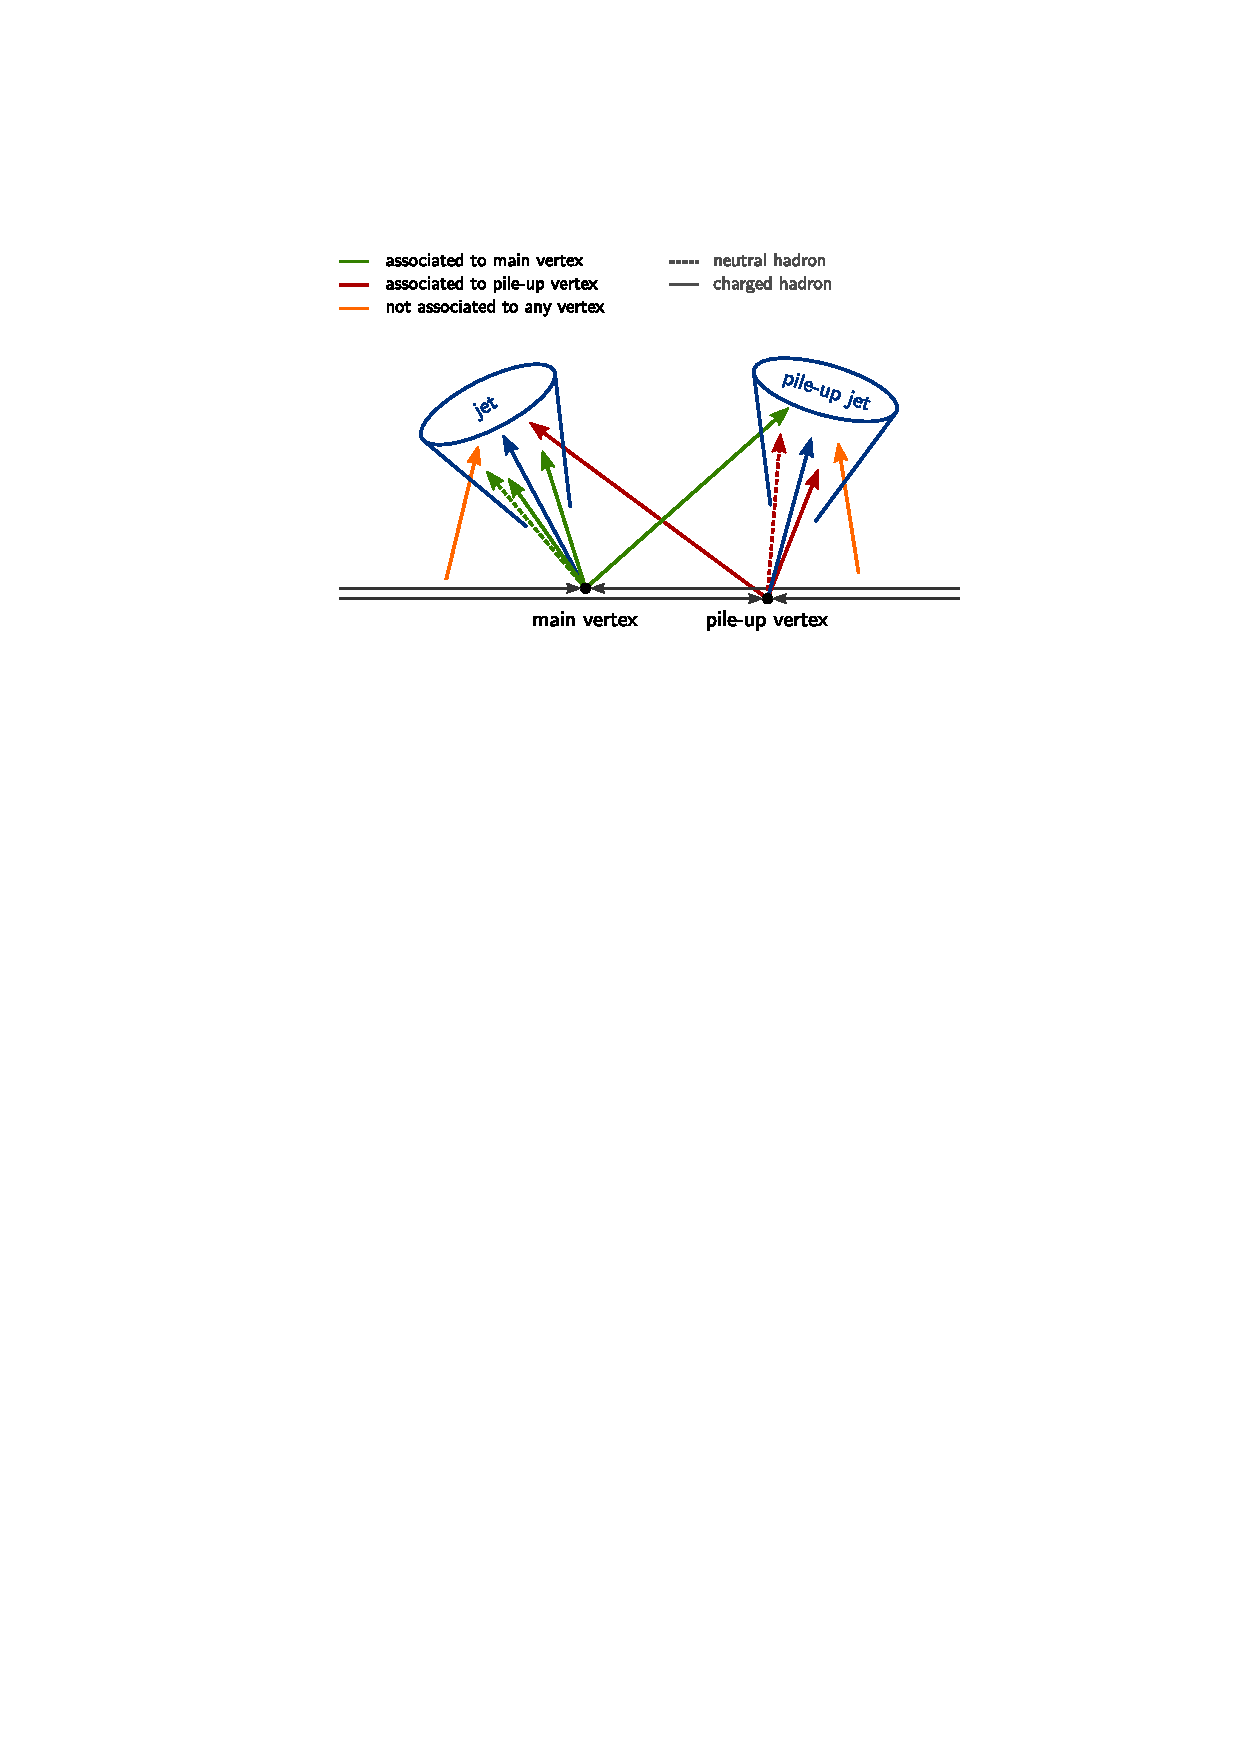
\includegraphics[width=.8\textwidth]{/home/anter/Desktop/Thesis/Figures/cropped_Pileup.pdf}\\
 \vspace*{5mm}
 \caption[Pileup Interactions]{In a proton-proton collision, the particles produced from the hard interaction are clustered into a jet. The hard interaction corresponds to the main vertex. The particles produced in the interactions other than the hard one, form a pileup jet\footnotemark.}
 \label{fig:pileup_d}
 \end{center}
\end{figure}
\footnotetext{Source : \url{http://cds.cern.ch/record/1747055}}

\section{The Compact Muon Solenoid}
The Compact Muon Solenoid (CMS) detector is a general purpose detector located at the interaction point 5 (P5) of the main LHC ring, near the village of Cessy in France. The name of CMS comes from its compact size with main emphasis on the detection of muons and enclosed within high solenoidal magnetic field. The CMS detector aims at identifying the different types of particles produced in proton-proton and heavy ion collisions and measuring their energies and momenta. This is achieved by concentric layers of different sub-detectors arranged in a cylindrical complex structure with 21.6 m length and 15 m diameter. The silicon-based tracker surrounds the the interaction point and forms the innermost layer. It is surrounded by a scintillating crystal electromagnetic calorimeter (ECAL) and a sampling hadron calorimeter (HCAL) which are enclosed inside the superconducting solenoid. Outside the magnet lies the large muon detectors embedded inside an iron yoke. 
\begin{figure}[!h]
\begin{center}
\vspace{2mm}
\hspace*{-6mm}
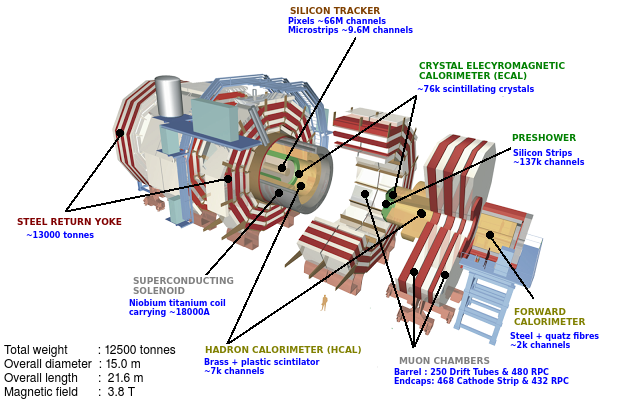
\includegraphics[scale = 0.98]{/home/anter/Desktop/Thesis/Figures/CMS_2_new.png}\\
\vspace*{5mm}
\caption[The three dimensional view of the CMS detector along with its sub-detector components.]{The three dimensional view of the CMS detector along with its sub-detector components\footnotemark.}
\label{fig:CMS}
\end{center}
\end{figure}
\footnotetext{Source : \url{https://orbiterchspacenews.blogspot.in/2013/04/cern-cms-prepares-for-future.html}}
The three dimensional view of the CMS detector along with its components is presented in Fig.~\ref{fig:CMS}. The CMS was constructed in parts at ground and assembled later on in the cavern. The components are easily accessible for upgrades or repairs as the detector can be opened up into movable slices. Figure~\ref{fig:CMS_front} shows the front view of the CMS detector differentiating individual components which contribute to event reconstruction. The path of reconstructed particles is represented by dashed (invisible track) and solid (visible track) lines for different particle classes : photons ($\gamma$), muons ($\mu^{\pm}$), electrons (e$^{-}$), neutrons (n) and charged hadrons (pions $\pi^{\pm}$).

\begin{figure}[!h]
\begin{center} 
\hspace*{-15mm}
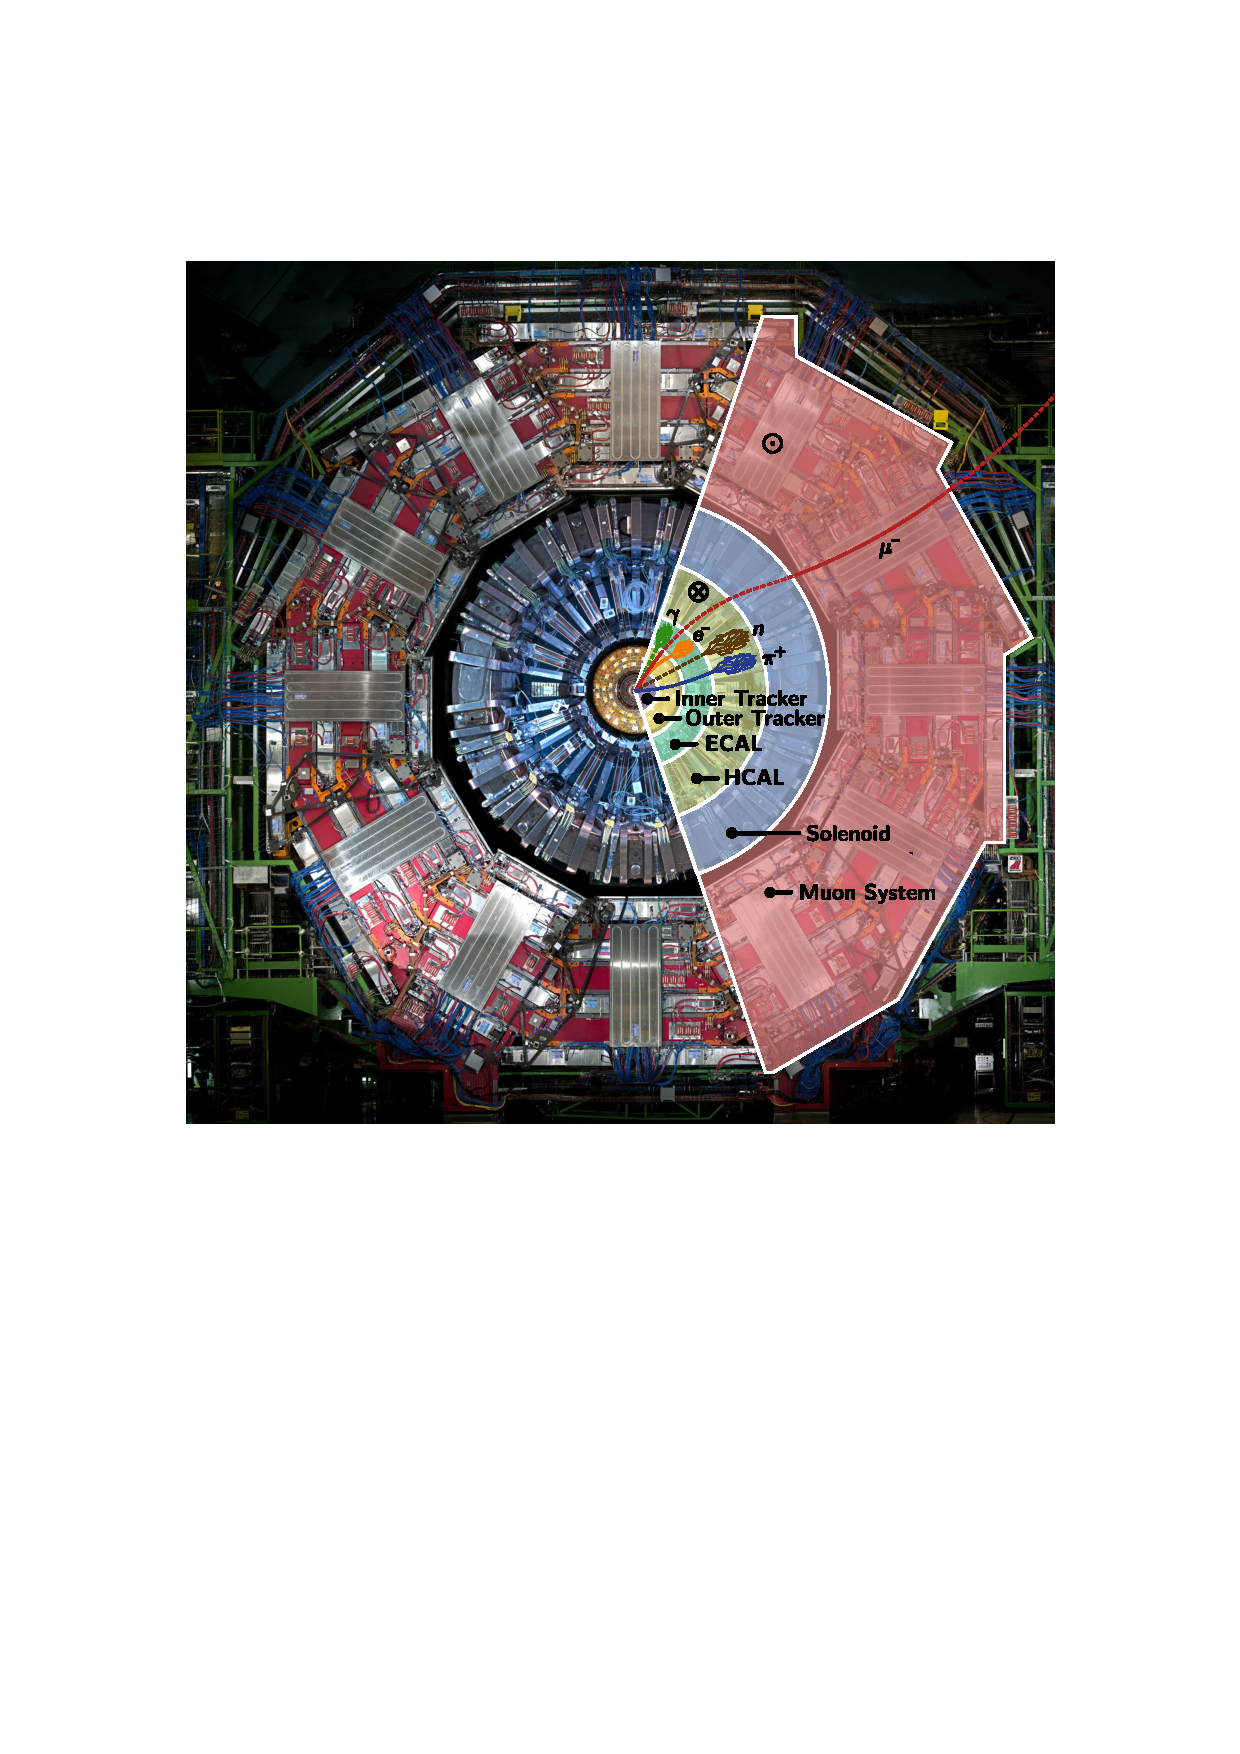
\includegraphics[scale = 0.55]{/home/anter/Desktop/Thesis/Figures/cropped_CMS_Front.pdf}
\caption[Front view of the CMS detector along with its components.]{Front view of the CMS detector along with its components : inner tracker, outer tracker, electromagnetic calorimeter, hadronic calorimeter, solenoid and muon system. The path of different particles detected by dedicated sub-detectors are shown by dashed (invisible track) and solid (visible track) lines. $\otimes$ and $\odot$ gives the direction of magnetic field inside the solenoid and in the return yoke, respectively. Taken from \cite{Ball:2007zza}.}
\label{fig:CMS_front}
\end{center}
\end{figure}

A brief overview of the CMS detector has been presented and the details of the its design as well as physics performance are available in Ref.~\cite{Bayatian:2006nff,Ball:2007zza}. Before going into the details of each sub-detector, first the CMS coordinate system is described in the next section.

\subsection{Coordinate System}
CMS uses right-handed coordinate system, illustrated in Fig.~\ref{fig:coordinate}, having origin at the nominal interaction point (IP) of the collision inside the detector. The $x$-axis points horizontally from the IP, towards the center of the LHC ring, the $y$-axis vertically upwards and the $z$-axis along the beam direction towards the Jura mountains. The radial coordinate in $x$-$y$ plane is denoted by $r$. 
\begin{figure}[!h]
\begin{center} 
\hspace*{-15mm}
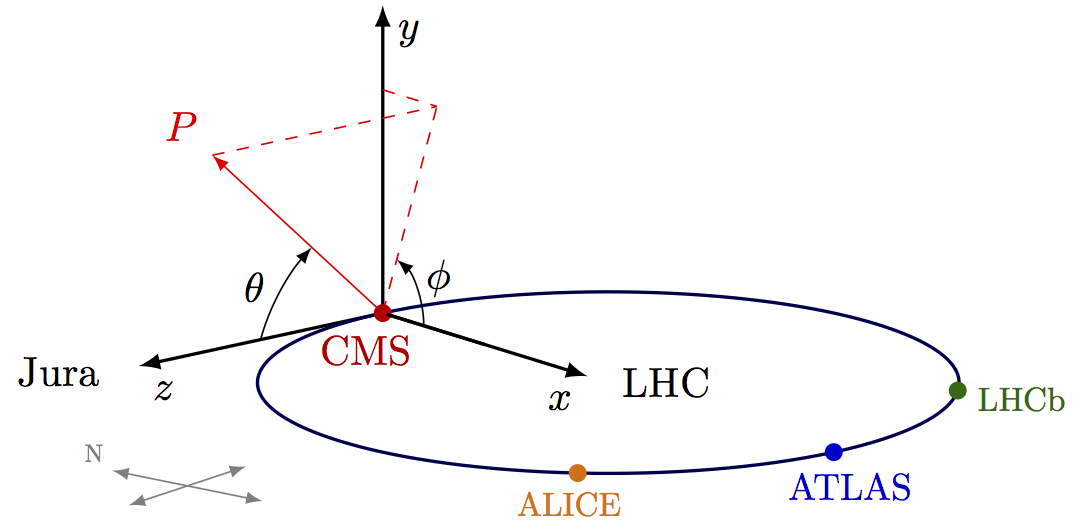
\includegraphics[scale = 1.5]{/home/anter/Desktop/Thesis/Figures/cms_coordinate_system.png}
\vspace{3mm}
\caption[The right-handed coordinate system used by the CMS detector.]{The right-handed coordinate system used by the CMS detector\footnotemark with origin at the interaction point (IP), $x$-axis points horizontally from the IP towards the center of the LHC ring, the $y$-axis vertically upwards and the $z$-axis along the beam direction towards the Jura mountains, $\phi$ as the azimuthal angle measured from the $x$-axis in the $x$-$y$ plane and $\theta$ as the polar angle calculated from the $z$-axis in the $z$-$y$ plane.}
\label{fig:coordinate}
\end{center}
\end{figure}
\footnotetext{Source : \url{https://wiki.physik.uzh.ch/cms/latex:example_spherical_coordinates}}
Following customary polar coordinate conventions : the azimuthal angle $\phi$ is measured from the $x$-axis in the $x$-$y$ plane as $\phi = {\rm tan^{-1}}(\frac{y}{x})$ where $\phi$ = 0 points to the \plusn $x$ axis and $\phi$ = $\pi$/2 points to the \plusn $y$ axis. The polar angle $\theta$, is calculated from the $z$-axis in the $z$-$y$ plane as $\theta~=~{\rm tan^{-1}}\big(\frac{x^2~\plus y^2}{2}\big)$ with $\theta$ = 0 corresponding to the \plusn $z$ direction and $\theta$ = $\pi$ to the -$z$ direction. The quantities pseudorapidity $\eta$ and the rapidity $y$ are preferred over the angles $\theta$ and $\phi$. The pseudorapidity and rapidity are given by Eq.~\ref{eq:pseudorap}. Both the quantities are equal for massless particles.
\begin{equation}
\begin{gathered}
\eta = -~{\rm ln}\bigg({\rm tan}\bigg(\frac{\theta}{2}\bigg)\bigg)\\
y = \frac{1}{2}~{\rm ln} \bigg(\frac{E~\plus p_z}{E - p_z} \bigg)
\end{gathered}
\label{eq:pseudorap}
\end{equation}
The difference between rapidities $\Delta y$ is invariant under longitudinal Lorentz boost whereas it does not hold for $\eta$. Hence $y$ is considered in this thesis. The angular distance between the two particles is defined by $\Delta R = \sqrt{(\Delta \eta)^2~\plus (\Delta \phi)^2}$. The momentum component transverse to the direction of beam \pt, is computed from the $x$- and $y$-components as \pt = $\sqrt{p^2_x~\plus p^2_y}$ and the transverse energy is given by $E_T$ = $E$ sin$\theta$. After introducing the CMS coordinate system, further the detector subsystems are described briefly in the following sections. A longitudinal section of the CMS detector in the $y$-$z$ plane, shown in Fig.~\ref{fig:CMS_quad}, locates the different sub-systems along with the superconducting solenoid.

\begin{figure}[!h]
\vspace*{2mm}
\begin{center} 
\hspace*{-5mm}
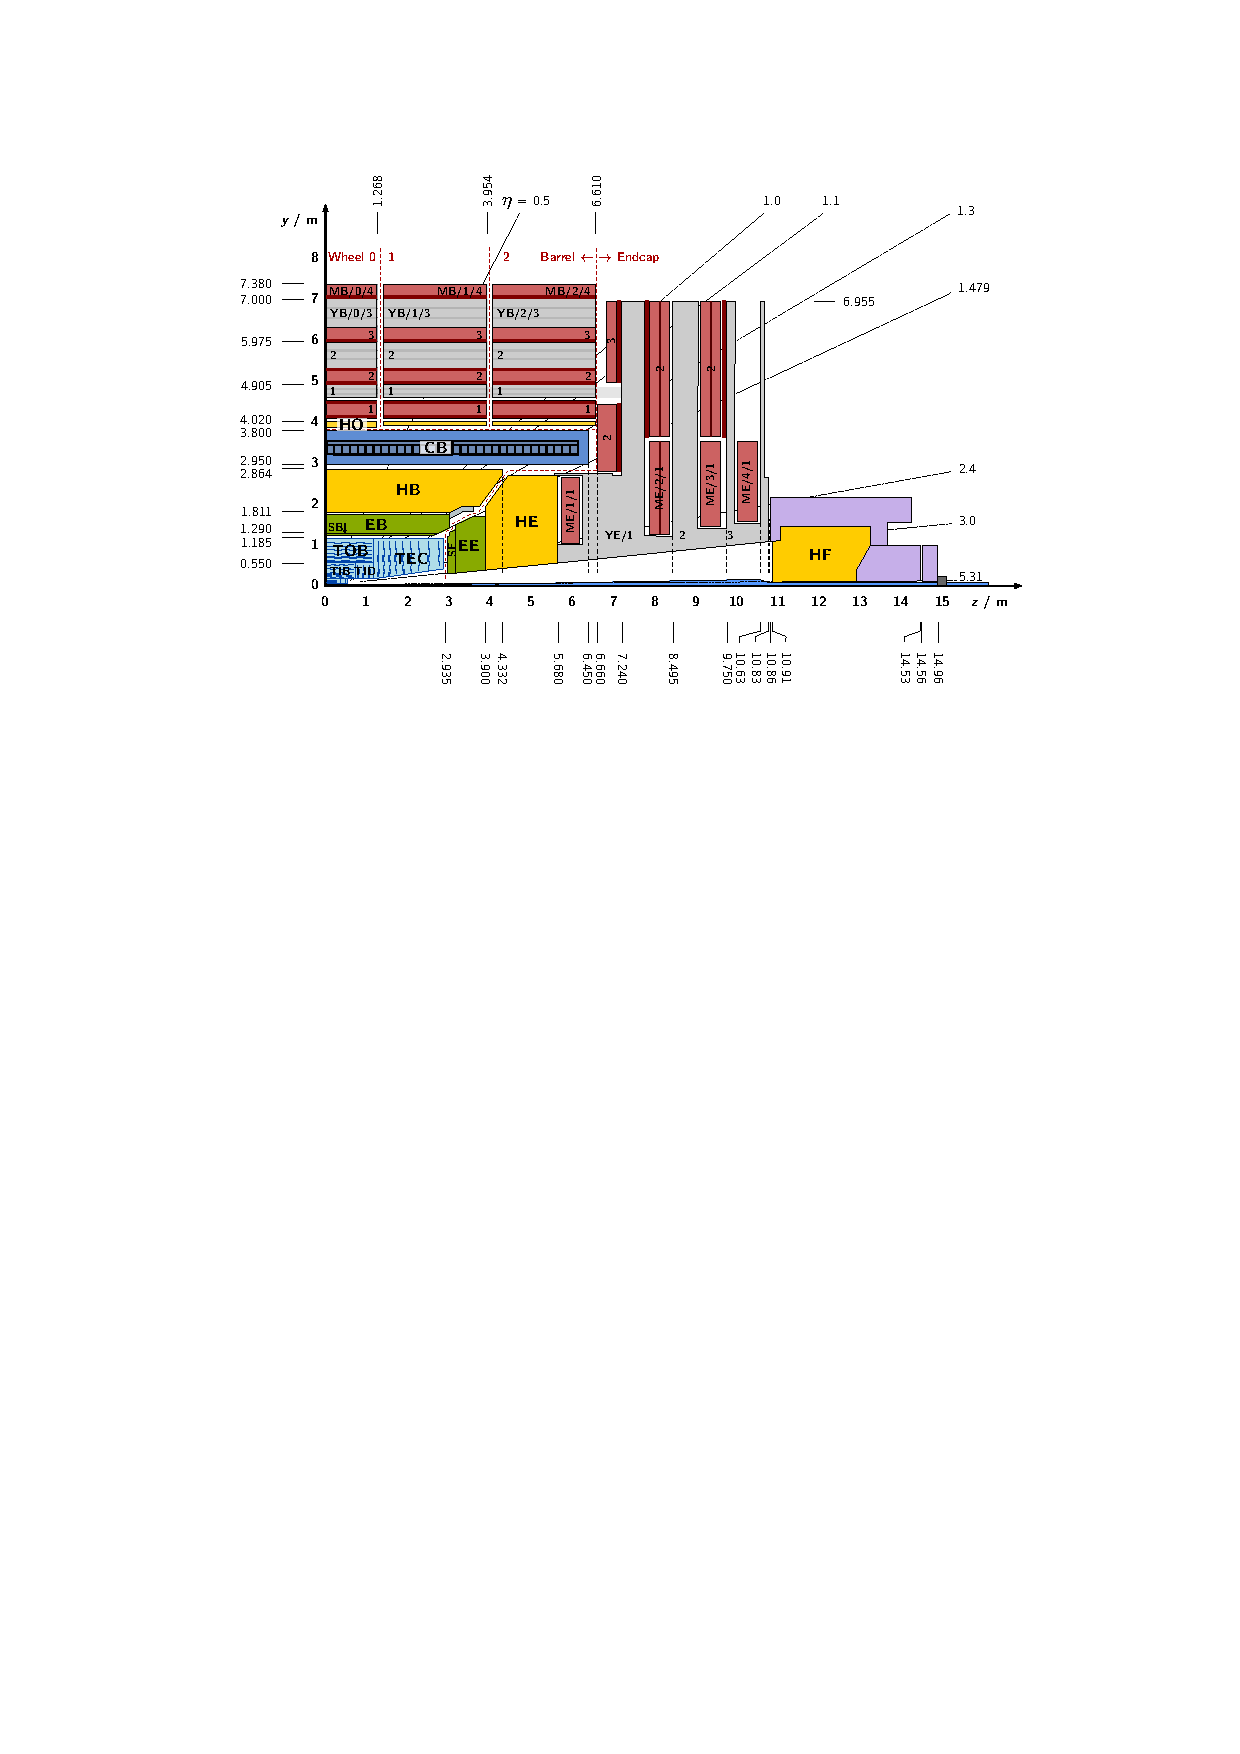
\includegraphics[scale = 1.1]{/home/anter/Desktop/Thesis/Figures/cropped_CMS_Quad.pdf}
\vspace{3mm}
\caption[Longitudinal section of the CMS detector in the $y$-$z$ plane.]{Longitudinal section of the CMS detector in the $y$-$z$ plane\footnotemark. It shows the tracking detector (TIB, TID, TOB, TEC) close to the nominal interaction point at (0,0), the electromagnetic (EB, EE) and hadronic (HB, HE, HO, HF) calorimeters. The coil of the solenoid magnet (CB) surrounds the inner barrel region. The iron return yoke (YB, YE) is interleaved with the muon chambers (MB, ME).}
\label{fig:CMS_quad}
\end{center}
\end{figure}

\subsection{Inner Tracker System}
The charged particles produced from the LHC collisions leave their trajectories as they move outward from the interaction point. The particle flux within the detector decreases as 1/$r^2$. So the tracks of the particles need to be measured as close to the collision point as possible and in a precise manner. The innermost tracking system of the CMS consisting of silicon detectors measures the hits of charged particles. It surrounds the interaction point and has a cylindrical volume of length of 5.8 m and a diameter of 2.5 m and covers a pseudorapidity range up to $|\eta|$ \ls 2.5. When charged particles pass through the silicon detector material, small ionization currents are produced which are detected as a hit. Such multiple hits when combined, reconstruct the track which gives the information about the direction and transverse momentum \pt of the charged particle. Silicon detectors have a much higher resolution in tracking charged particles as compared to the older ones such as cloud chambers or wire chambers.\footnotetext{Source : \url{http://cds.cern.ch/record/1747055}} CMS inner tracking system shown in Fig.~\ref{fig:tracker} consists of two sub-systems :\\ \newline 
{\bf Pixel Detector -} A pixel detector lying close to the beam pipe have three co-centric barrel layers at radii of 4.4, 7.3 and 10.2 cm from the beam pipe. It has two disks of pixel modules on each side of barrel. At the LHC design luminosity of 10$^{34}$ cm$^{-2}$s$^{-1}$, about 1000 particles from more than 20 overlapping proton-proton interactions traverse through the tracker for each bunch crossing, i.e. every 25 ns. The size of each pixel is 100 $\micro$m $\times$ 150 $\micro$m which gives an average occupancy of 10$^{-4}$ per bunch crossing. By taking an advantage of the large Lorentz effect, the pixel tracker has a resolution of 10 $\micro$m $\times$ 20 $\micro$m needed for a precise determination of the primary and secondary vertices and the required momentum resolution. \\ \newline
{\bf Strip Detector -} After coming out of the pixel detector the charged particles pass through ten layers of silicon strip detectors, reaching out to a radius of 130 cm. The silicon strip detector consists of four inner barrel (TIB) layers assembled in shells with two inner endcaps (TID), each composed of three small discs. The outer barrel (TOB) consists of six concentric layers. Finally two endcaps (TEC) close off the tracker. Each part has silicon modules designed differently for its place within the detector. The strip detector measures the particle tracks with a reduced resolution of 23 $\micro$m reflecting the smaller particle flux at larger distances from the interaction point.
\begin{figure}[!h]
\begin{center} 
\vspace*{2mm}
\hspace*{-6mm}
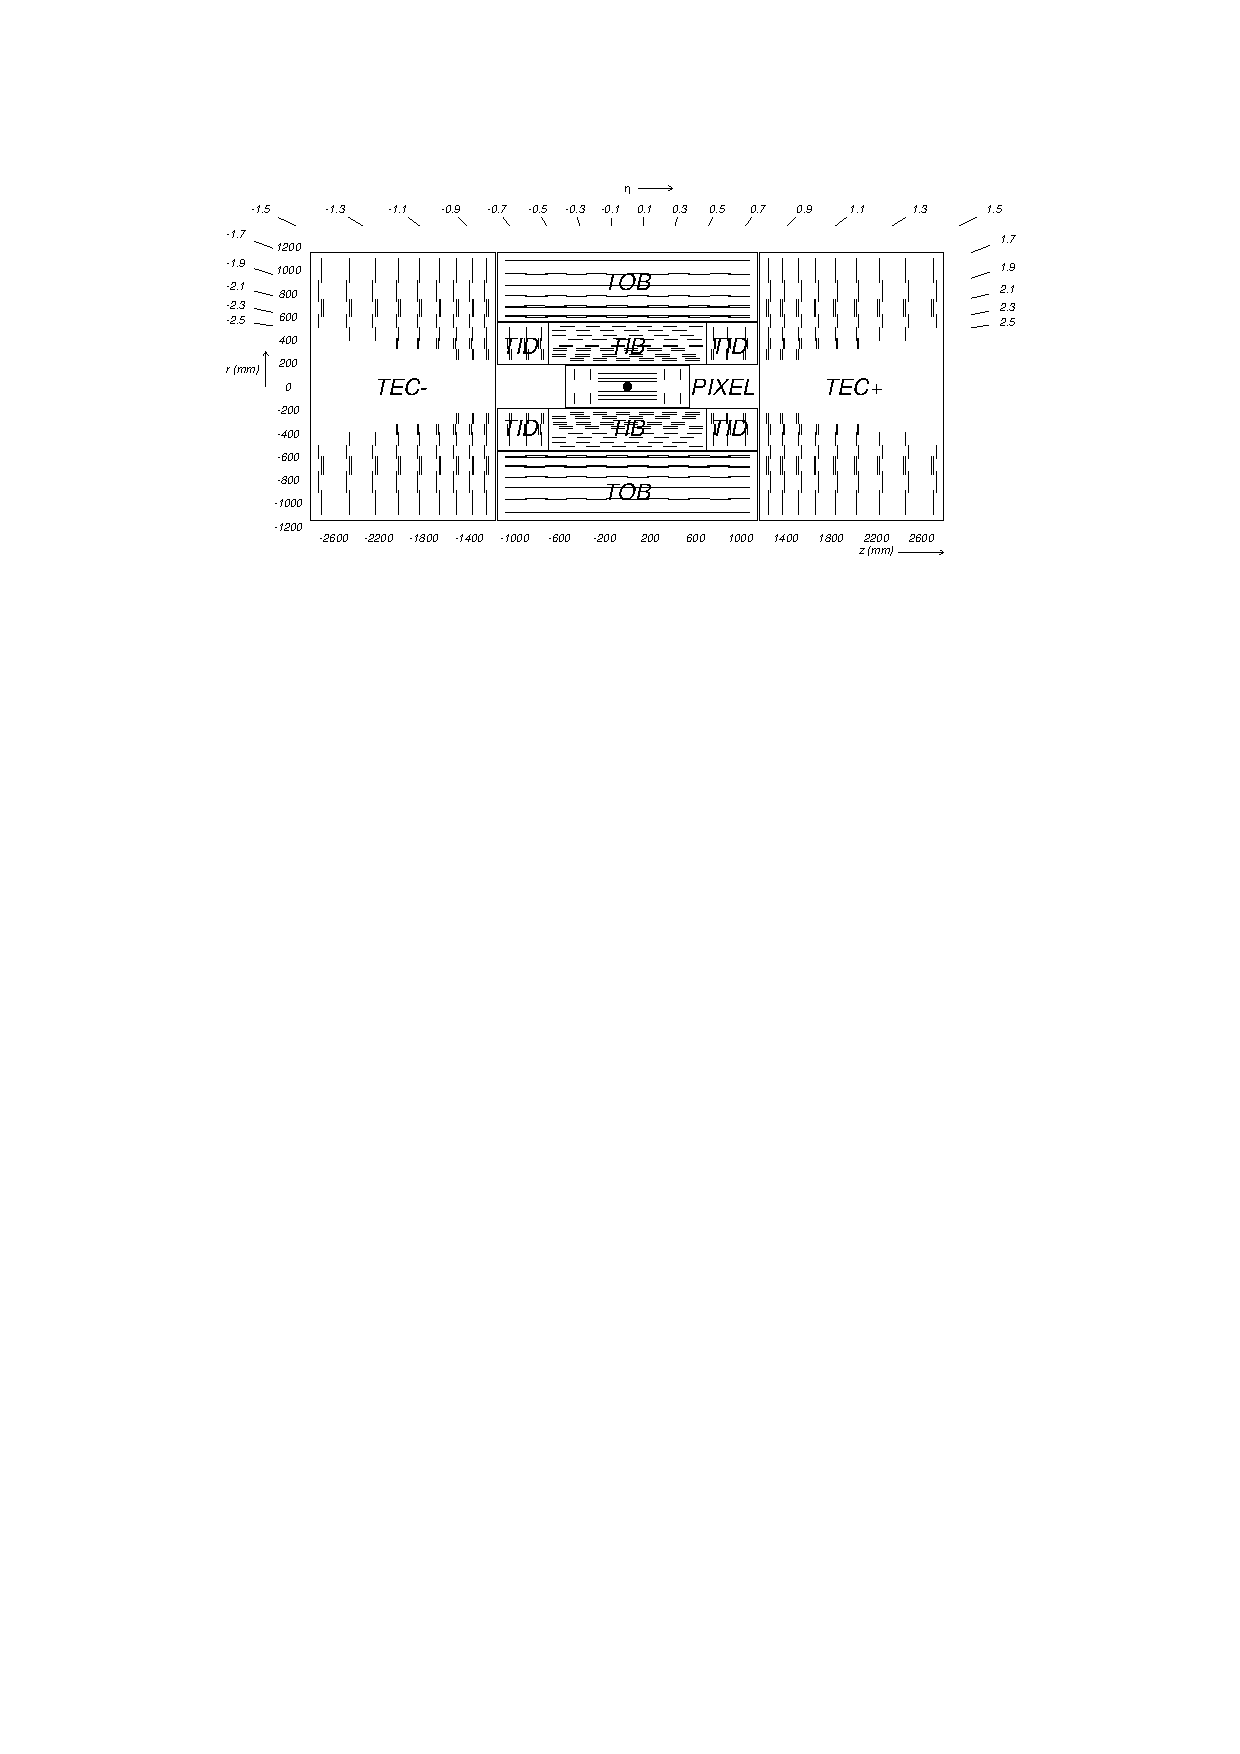
\includegraphics[scale = 1.1]{/home/anter/Desktop/Thesis/Figures/cropped_Tracker.pdf}\\
\caption[The longitudinal section of the inner tracking system.]{The longitudinal section of the inner tracking system consisting of the silicon pixel detector and the silicon strip detector is shown in $r$-$z$ plane. The silicon strip detector has four components : The Tracker Inner Barrel (TIB) complemented by the Tracker Inner Disks (TID) which are further surrounded by the Tracker Outer Barrel (TOB) in barrel region. Tracker End Cap (TEC) covers high $\eta$ ranges up to $\eta$ = 2.5. Taken from \cite{Chatrchyan:2008aa}.}
\label{fig:tracker}
\end{center}
\end{figure}
The active silicon area of CMS tracker is about 200m$^{2}$ which makes it the largest silicon tracker. Along with the measurement of tracks, the energy also needs to be measured for which the calorimeters are present outside the tracker. The tracker should interfere with the particles to a minimum extent so that their momentum can be measured precisely but to measure their energy, they are required to interact with the calorimeters fully.

\subsection{Electromagnetic Calorimeter}
The electromagnetic calorimeter (ECAL) is a homogeneous and hermetic calorimeter used to slow down the produced photons and electrons/positrons and measure their energy by absorb them into the detector material. ECAL consists of 61200 lead tungstate (PbWO$_4$) crystals in the barrel part and 7324 crystals in each of the two endcaps. PbWO$_4$ is a very dense material with a short radiation length of X$_0$ = 0.89 cm and covers the pseudorapidity up to $|\eta|$ \ls 3.0. The particles interact with matter and produce electromagnetic shower through the subsequent processes of bremsstrahlung and electron-positron pair production. The energy of the particles deposited by Compton scattering and the photoelectric effect causes excitation of the material atomic state and the emission of photons. These photons are detected by silicon avalanche photo diodes (APDs) in the barrel region and vacuum phototriodes (VPT) in the end-cap region. The number of created photons gives the direct measure of energy of the incident particle. The incorporation of oxygen makes it highly transparent and enables to emit scintillation light. The small Moli$\grave{e}$re radius of 2.19 cm gives a fine granularity. These properties leads to compact size of ECAL and can be placed easily within the solenoid magnet. 

Figure~\ref{fig:ecal} presents a geometric view of ECAL in the $y$-$z$ plane showing the arrangement of different parts of ECAL 
: the ECAL barrel (EB) extending up to $|\eta|$ \ls 1.479 using more than 60000 crystals and ECAL endcaps (EE) covering the region 1.479 \ls $|\eta|$ \ls 3.0 with an additional 15000 crystals. The preshower detectors (ES) made of lead absorbers and silicon detectors are put in front of the endcaps to distinguish high energetic single photons from low energetic photon pairs originating from neutral pions decays.

\begin{figure}[!h]
\begin{center}
\vspace*{3mm} 
\hspace*{-5mm}
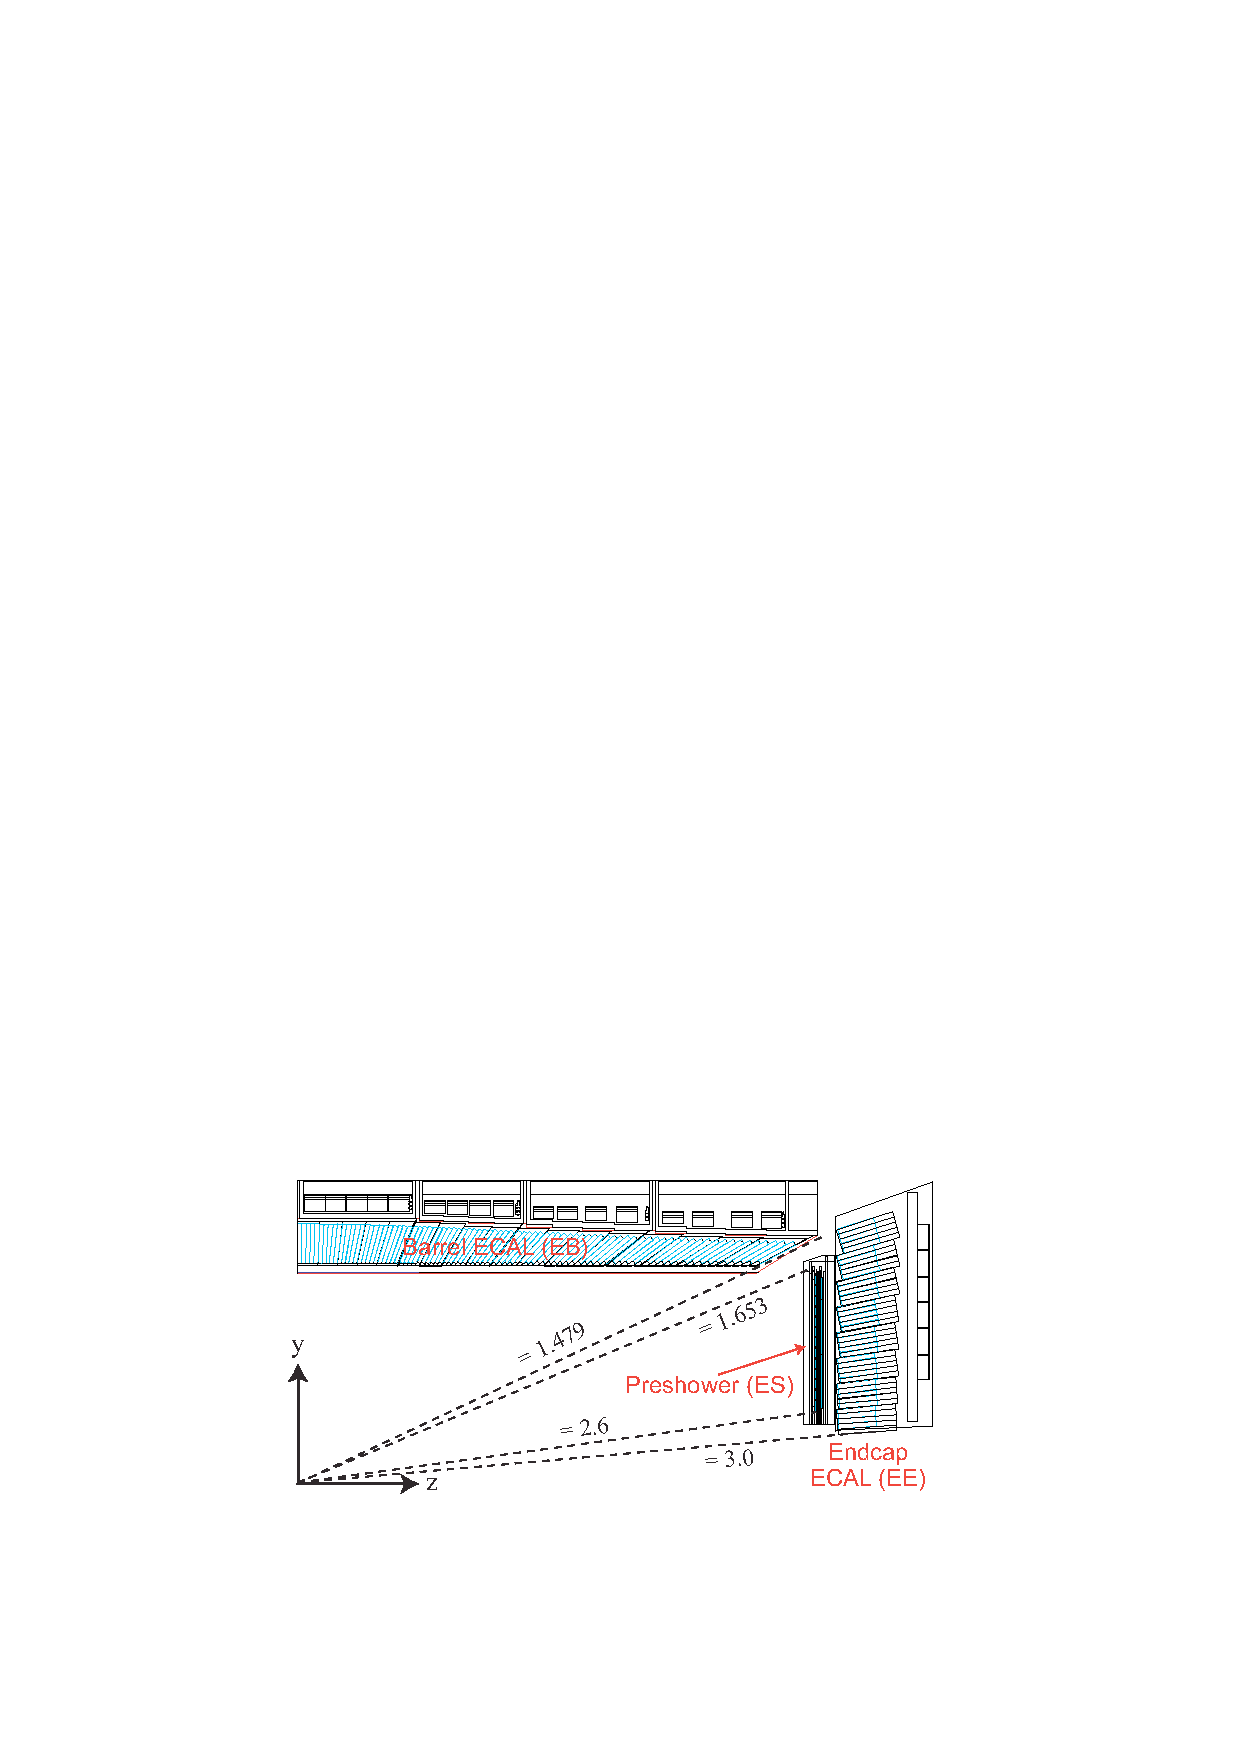
\includegraphics[scale = 1.2]{/home/anter/Desktop/Thesis/Figures/cropped_ECAL.pdf}\\
\vspace*{2mm}
\caption[A geometric view of one quarter of the electromagnetic calorimeter (ECAL) in $y$-$z$ plane.]{A geometric view of one quarter of the electromagnetic calorimeter (ECAL) in $y$-$z$ plane showing the arrangement of sub-modules covering the barrel region (EB) and the endcaps (EE). ECAL is complemented with preshower detector (ES) mounted in front of the endcaps. Taken from \cite{Bayatian:2006nff}.}
\label{fig:ecal}
\end{center}
\end{figure}

The relative energy resolution of the ECAL has been measured to be \cite{Adzic:2007mi} :

\begin{equation}
{\rm \bigg(\frac{\sigma(E)}{E}\bigg)^2 = \bigg(\frac{2.8\%}{\sqrt{E}}\bigg)^2 \plus \bigg(\frac{12\%}{E}\bigg)^2 \plus \bigg(0.30\%\bigg)^2}
\end{equation}
where E is the energy in GeV. The first term is the stochastic component caused by fluctuations in lateral shower containment and in the energy deposited in the preshower absorber. The second term is the contribution by noise and the last is the constant term comes from the non-uniformity of the longitudinal light collection, inter-calibration errors, and leakage of energy from the back of the crystal.

\subsection{Hadronic Calorimeter}
At CMS, the major fraction of the produced particles in proton-proton collisions is hadrons. The combined CMS calorimeter system measures directions and energies of quarks, gluons and neutrinos by measuring the energy and direction of particle jets. The neutral hadrons do not leave track and hence their energy is measured by taking into account the missing transverse energy (\ETmiss). The determination of \ETmiss is a crucial tool in searching the new particles and phenomena. The hadron calorimeter (HCAL) are particularly important in the identification of hadron jets, neutrinos as well as electrons, photons and muons in conjunction with the ECAL and the muon system. Hence HCAL is an essential sub-system of the CMS detector and contributes to most of CMS's physics studies.

HCAL is a sampling calorimeter installed inside the solenoid coil. It is made up of non-magnetic brass absorber having a short interaction length of $\lambda_I$ = 16 cm interleaved with plastic scintillators having wavelength-shifting (WLS) fibres as readout. The hadrons produced with high energy showers a large number of pions and nucleons by inelastic interactions. The hadronic shower spreads more than the electromagnetic showers because of large transverse momentum of the secondary particles. As the energy of the particles is lower than a certain threshold, the ionization and low-energy hadronic processes come into play. The active scintillation material gets excited and emits blue-violet light. 
\begin{figure}[!h]
\begin{center}
\vspace*{3mm} 
\hspace*{-5mm}
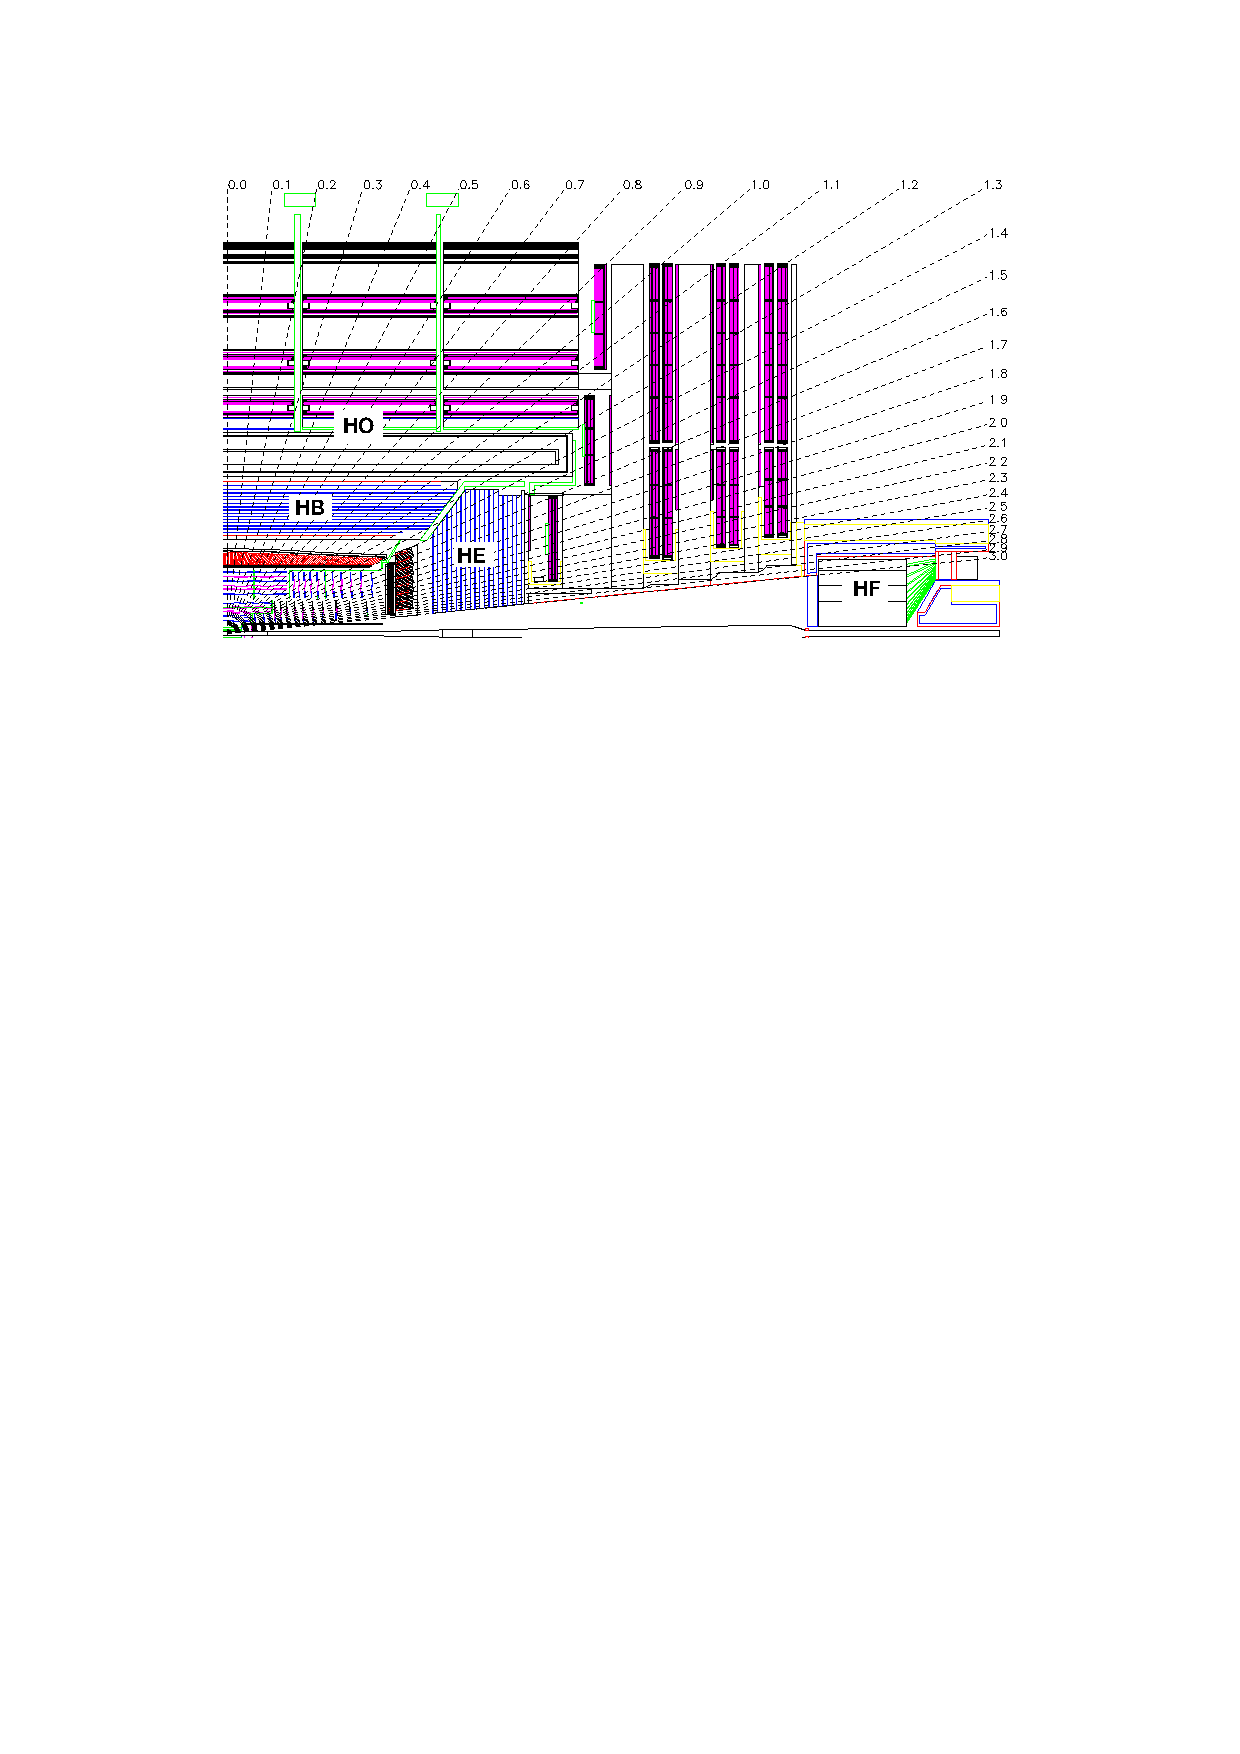
\includegraphics[scale = 1.]{/home/anter/Desktop/Thesis/Figures/edited_cropped_HCAL.pdf}\\
\vspace*{4mm}
\caption[Longitudinal view of one quarter of the hadronic calorimeter (HCAL) detector in $r$-$\eta$ plane.]{Longitudinal view of one quarter of the hadronic calorimeter (HCAL) detector in $r$-$\eta$ plane showing its different parts : hadron barrel (HB), hadron outer (HO), hadron endcap (HE) and hadron forward (HF). Taken from \cite{Chatrchyan:2008aa}.}
\label{fig:hcal}
\end{center}
\end{figure}
All scintillators are connected to photodiodes using wavelength shifters which read out the signals and pass them to the data acquisition system. The longitudinal view of one quarter of the HCAL presented in Fig.~\ref{fig:hcal} shows the different parts : \\\newline
{\bf Hadron Barrel -} The hadron barrel (HB) is divided into two identical half barrel sections on either side of the interaction point. Each half barrel is made of 18 azimuthal wedges which are further divided into four azimuthal sectors each giving a granularity of $\Delta\phi$ = 0.087. In $z$ direction, the plastic scintillators are divided into 16 intervals of granularity $\Delta\eta$ = 0.087. HB covers the region up to $|\eta|$ \ls 1.305 and overlaps with endcaps for 1.305 $\leq~|\eta|~\leq$ 1.392. Since HB has the highest resolution $(\Delta\eta~\times~\Delta\phi = 0.087~\times~0.087$), it constitute the optimal region for a data-driven calibration of the jet energy scale. The thickness of the HCAL amounts to 7-11 interaction lengths and which should sufficient enough to stop nearly all hadrons in the calorimeter.\\\newline
{\bf Hadron Outer -} The total amount of material in barrel region to absorb the hadronic shower is not sufficient. This requirement is fulfilled by placing an outer hadron (HO) calorimeter as a tail catcher on top of the coil of the magnet. The HO utilizes the solenoid coil as an additional absorber equal to 1.4/sin$\theta$ interaction lengths and measures the tails of hadron showers penetrating the HB and the coil. Since the HO is physically located inside the muon system, it is strongly constrained by its geometry. The muon system is subdivided into 5 rings along the $z$-axis. Each of these rings is 2.536 m wide in $z$-direction and the HO is placed as first sensitive layer in these rings, with a scintillator thickness of 10 mm. The central ring ($\eta$ = 0) has two scintillator layers placed on each side of 19.5 cm thick iron layer.\\ \newline
{\bf Hadron Endcap -} The hadron endcaps (HE) extends the pseudorapidity range up to $|\eta|$ \ls 3.0, a region containing about 34\% of the particles produced in the final state The granularity in $\Delta\eta~\times~\Delta\phi$ is 0.087 $\times$ 0.087 up to $|\eta|$ \ls 1.6 and 0.17 $\times$ 0.17 for $|\eta|$ \gr 1.6. The usage of non-magnetic material in order to not disturb the magnetic field and the close distance to the beam line were the main challenges faced during the construction of the HE. The continuous radiation damages decrease the detector response which need to be corrected and monitored at regular intervals. \\ \newline
{\bf Hadron Forward -} The hadron forward (HF) calorimeter lies 2.8 \ls $|\eta|$ \ls 5.2 region and is placed more closer to the beam pipe at distance of $z$ = $\pm$11.2 m from the interaction point. It is essentially a cylindrical steel structure with an outer radius of 130.0 cm which is azimuthally subdivided into 36 20$\degree$ modular wedges. The HF is made of 5 mm thick grooved steel plates which have quartz fibers inserted into the grooves. The fibres run parallel to the beam line which are bundled to form 0.175 $\times$ 0.175 ($\Delta\eta~\times~\Delta\phi$) towers. HF detects the jets with very high $\eta$ and the hadronization products of the beam remnants. It is built using iron absorbers and quartz fibers as active material, which measures the emitted Cerenkov light and produces the signal in the photomultipliers (PMT).

%HCAL provides the energy and direction measurements of the jets in conjunction with ECAL system. It measures the total visible and missing transverse energy due to hermetic coverage.
The relative hadronic energy resolution of the barrel HCAL and ECAL combination can be parametrized as :
\begin{equation}
{\rm \bigg(\frac{\sigma(E)}{E}\bigg)^2 = \bigg(\frac{a}{\sqrt{E}}\bigg)^2 \plus b^2}
\end{equation}
with a stochastic term a and a constant term b. These values have been measured \cite{Chatrchyan:2009ag} as a = (0.847$\pm$0.016) $\sqrt{\rm GeV}$ and b = 0.074 $\pm$ 0.008 whereas for HF the measured values are a = 1.98 $\sqrt{\rm GeV}$ and b = 0.09.

\subsection{Superconducting Magnet}
The superconducting magnet is the key feature of the CMS detector which is 13m long and 6m in diameter. Its refrigerated superconducting high-purity aluminium-stabilized niobium-titanium coils cooled at 4 Kelvin produces a magnetic field of 4 Teslas (T). The magnet will run at 3.8 T in order to maximize its lifetime. This intense solenoidal field makes the compactness and cylindrical symmetry of the detector possible. The magnet is placed between the calorimeters and the muon system. The solenoidal magnetic field parallel to the beam bends the tracks of the high momentum charged particles in the transverse plane. The curvature of the trajectory increases with the strength of the magnetic field which make possible to determine the transverse momentum more precisely. The magnet is complemented by a $\sim$10000 tonnes iron yoke which returns the magnetic field at 2 T.

\subsection{Muon System}
As the name suggests, the detection of muons is of central importance to CMS. Only the muons and neutrinos, out of all the known stable particles, pass through the calorimeter without depositing most or all of their energy. They interact very little with matter and can travel long distances through the dense matter. The charged muons can be detected by having an additional tracking system outside the calorimeters whereas the neutrinos are practically undetectable as they escape completely without being tracked in any of the layers. Their presence can be detected from the missing energy carried by them. The CMS muon system is installed outside calorimeters in the iron return yoke of the magnet. The muon system perform the muon identification, momentum measurement and triggering. Good muon momentum resolution and trigger capability are enabled by the high-field solenoidal magnet and its flux-return yoke. The latter also serves as a hadron absorber for the identification of muons. The CMS muon system is designed to have the capability of reconstructing the momentum and charge of muons over the entire kinematic range of the LHC. The muon system shown in Fig.~\ref{fig:muon} consists of three types of gaseous particle detectors : \\ \newline
\begin{figure}[!h]
\begin{center}
\vspace*{3mm} 
\hspace*{-5mm}
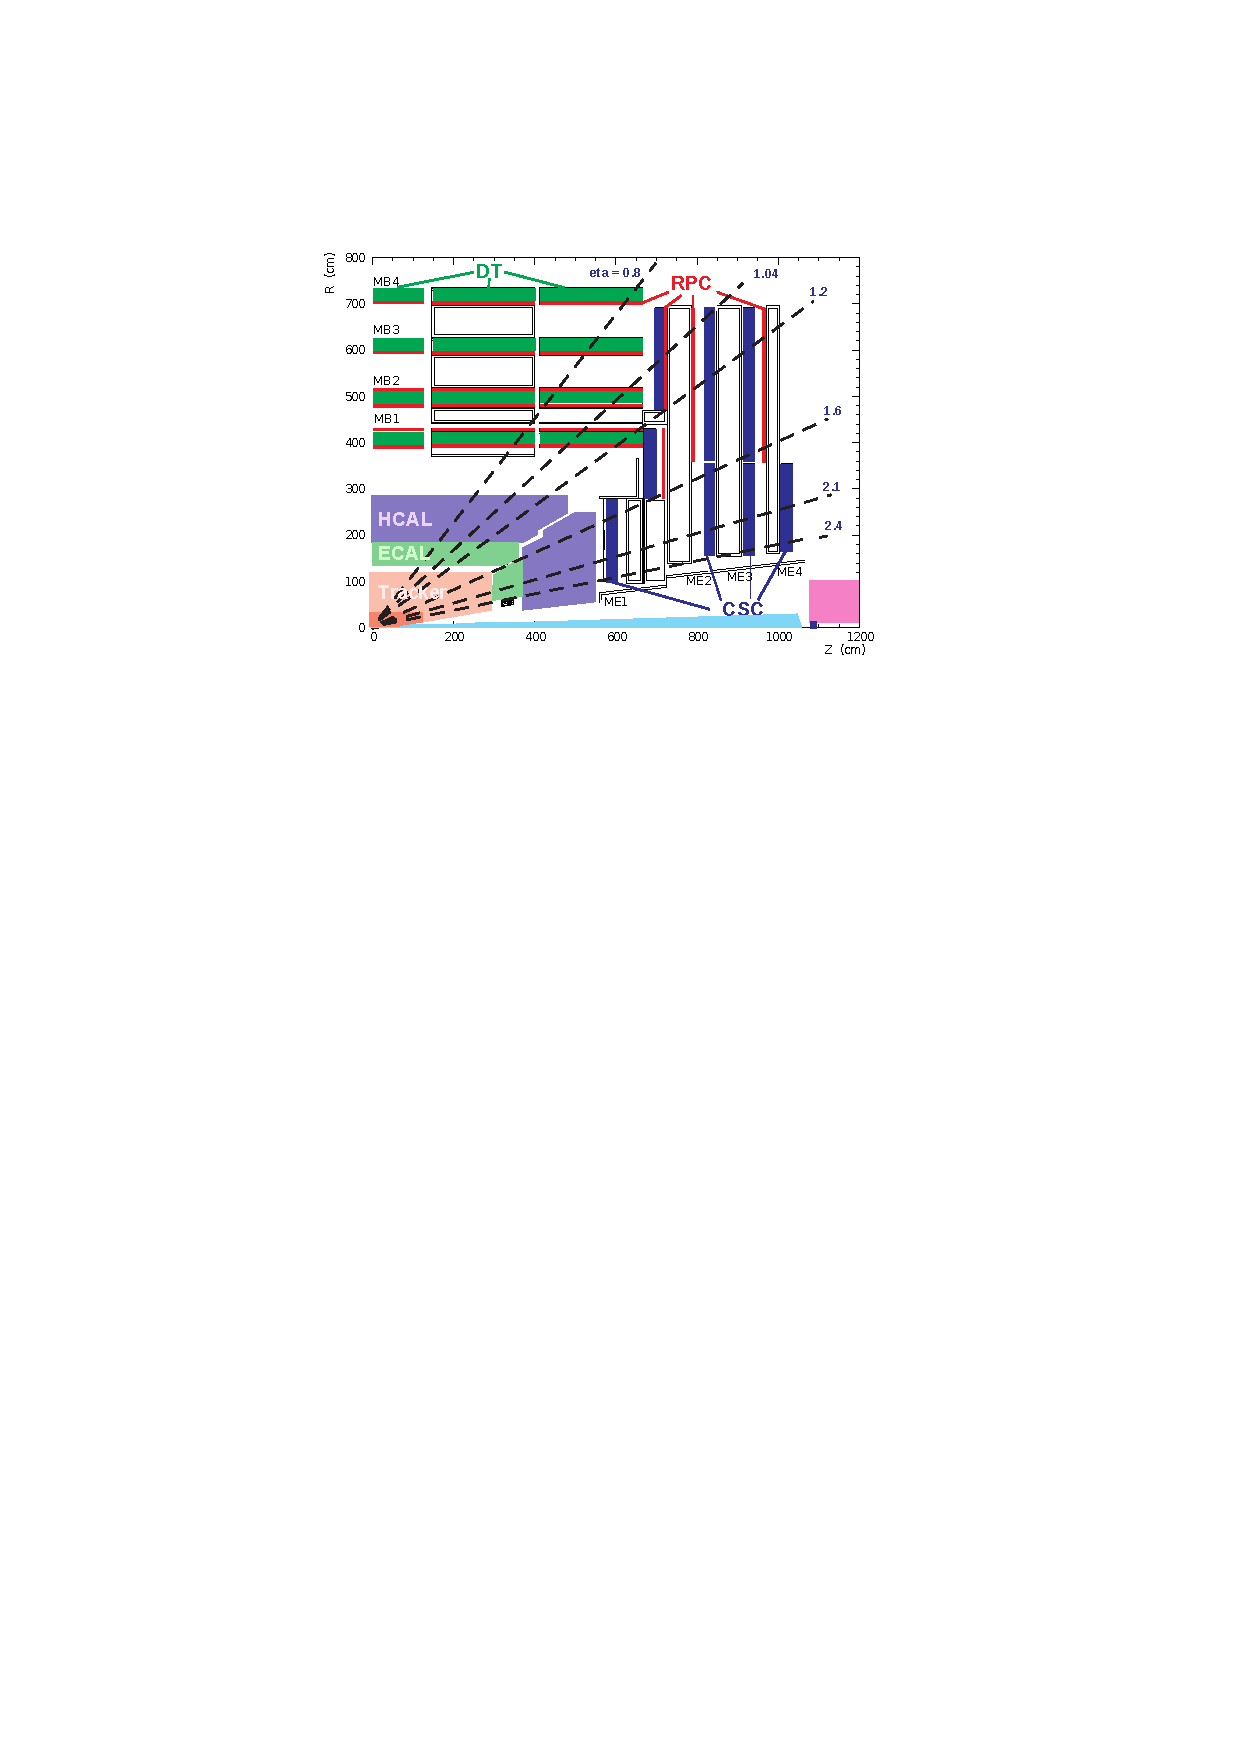
\includegraphics[scale = 1.4]{/home/anter/Desktop/Thesis/Figures/cropped_Muon.pdf}\\
\vspace*{4mm}
\caption[A longitudinal view presenting the location of the three muon sub-systems.]{A longitudinal view presenting the location of the three muon sub-systems : four Drift Tube (DT) stations in the barrel (MB1-MB4, green), four stations of Cathode Strip Chambers (CSC) in the endcap (ME1-ME4, blue), and the Resistive Plate Chambers (RPC) stations (red)\footnotemark.}
\label{fig:muon}
\end{center}
\end{figure}
{\bf Drift Tube -} 
The muon barrel (MB) detector has four concentric layers of drift tube (DT) chambers inside the iron yoke which covers the region up to $|\eta|$ \ls 1.2. DT stations are distributed into 5 wheels along the $z$ direction. Each wheel is divided into 12 sectors, each covering a 30$\degree$ azimuthal angle. The DTs are aluminium tubes of 2.5 m of length and 4.2 $\times$ 1.3 cm$^{2}$ of area, filled with gas mixture ( 58\% Ar \plus 15 \% CO$_{2}$). \\ \newline \footnotetext{Source : \url{https://arxiv.org/abs/1209.2646}}
{\bf Cathode Strip Chambers -} In the forward region, the muon and background flux is higher. So cathode strip chambers (CSC) are preferred because of their fast response time, radiation tolerance and fine segmentation. The four stations of CSCs are installed in each end cap covering in total the region of 0.9 \ls $|\eta|$ \ls 2.4. Each CSC is trapezoidal in shape and consists of 6 gas gaps, each gap having a plane of radial cathode strips and a plane of anode wires running almost perpendicularly to the strips. \\ \newline 
{\bf Resistive Plate Chambers -} Both DT and CSC are accompanied by resistive plate chambers (RPC) which are double-gap chambers, operated in avalanche mode to ensure good operation at high rates. They help to resolve ambiguities in attempting to make tracks from multiple hits in a chamber and provide additional points for determination of a muon trajectory. They provide fast response to the trigger system which is described in the following section.
 
\subsection{Trigger and Data Acquisition System}
The proton-proton collisions (events) take place at high interaction rates at LHC. In the 2012 run period, at beam crossing frequencies of 25 ns there are 40 million bunch crossings per second with an average of around 20 collisions per bunch crossing. Both the collision and the overall data rates are much higher than the rate at which the information can be stored. So a dramatic rate reduction has to be achieved which is possible with an efficient trigger system by retaining interesting signal events and rejecting background events. The decision of accepting or rejecting an event has to be performed very quickly and it is based on signals of certain physics objects inside the detector.
CMS has a two-level complex trigger system : \\\newline
{\bf Level-1 Trigger -} The Level-1 (L1) trigger system is based on custom electronics which stores the events at maximum rate of 100 kHz and then forward them to the next level triggers. The L1 system uses only coarsely segmented data from calorimeter and muon detectors, while holding all the high-resolution data in pipeline memories in the front-end electronics. Figure~\ref{fig:L1} shows the work flow of the L1 trigger system. 
\begin{figure}[!h]
\begin{center}
\vspace*{3mm} 
\hspace*{-5mm}
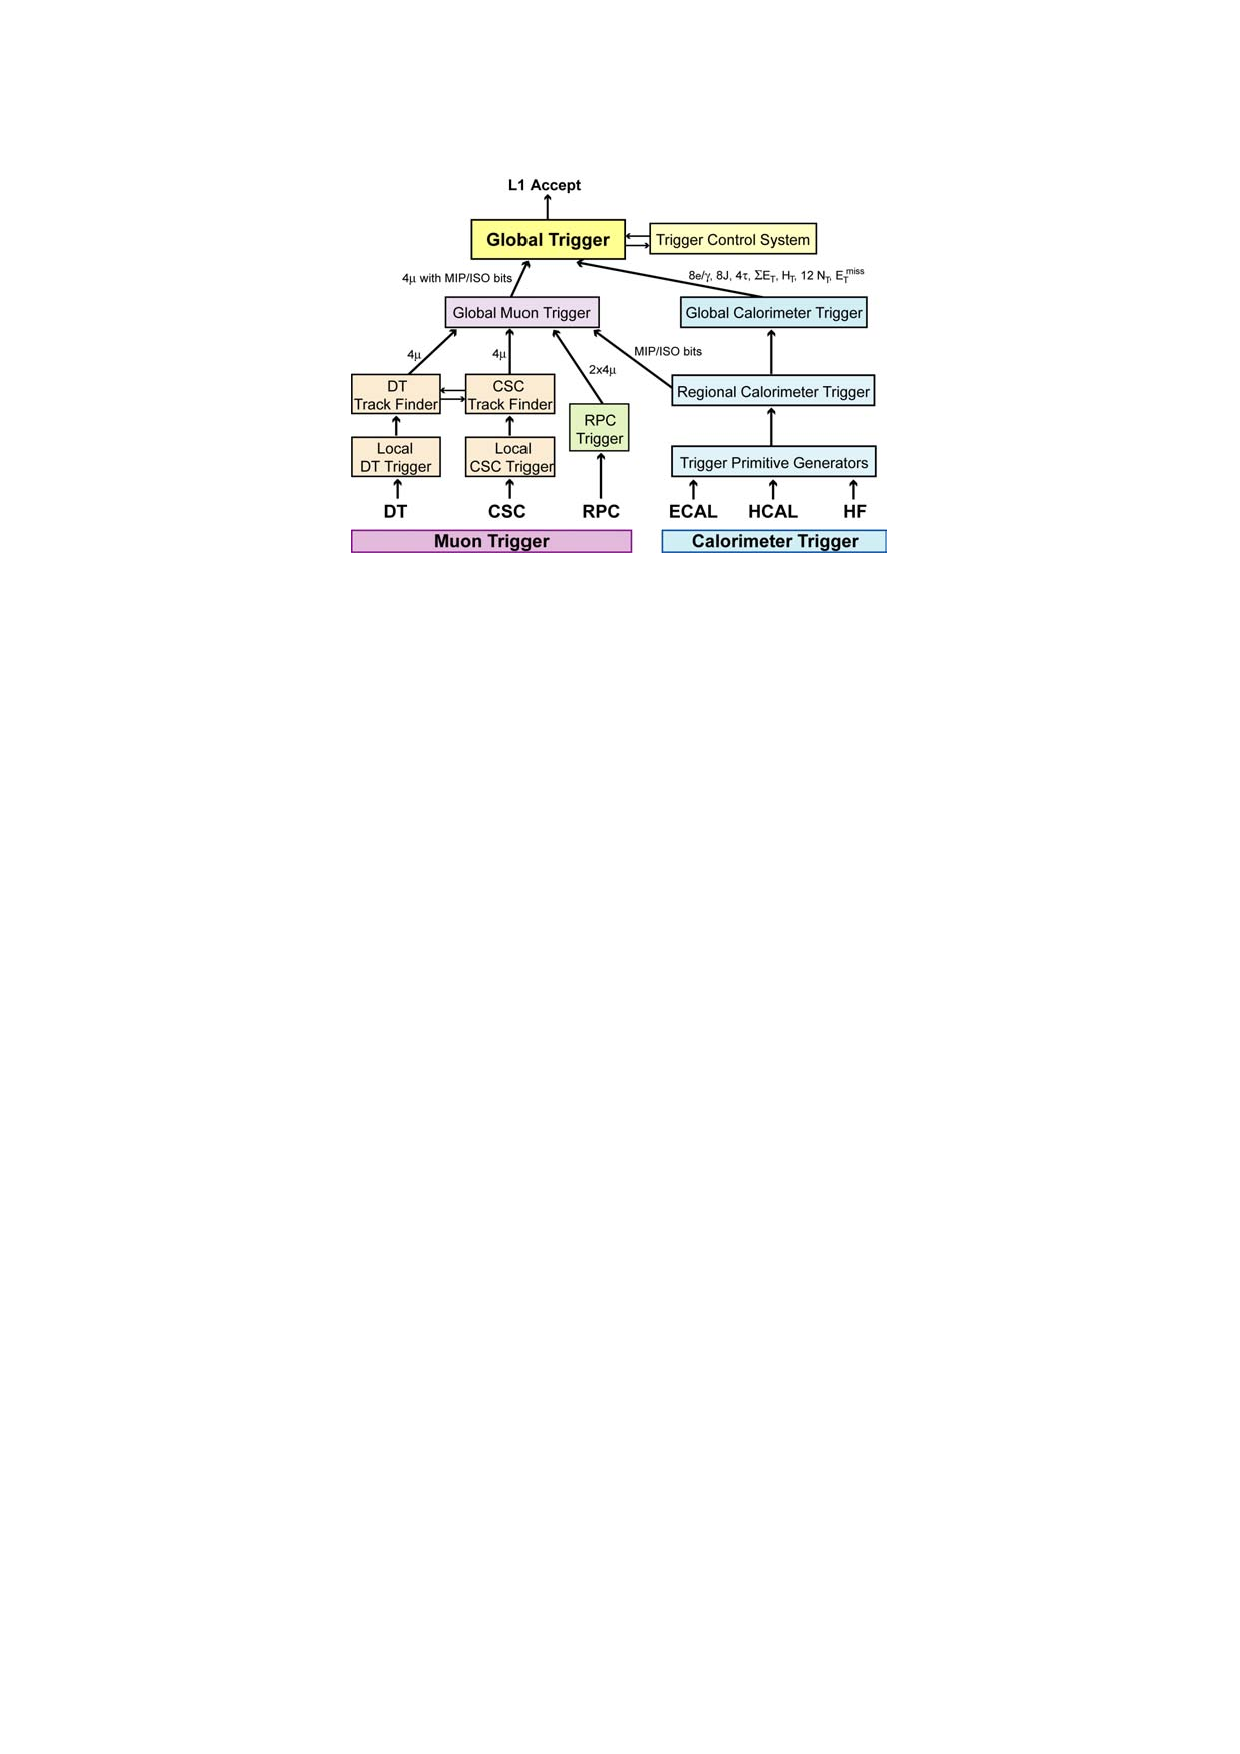
\includegraphics[scale = 1.5]{/home/anter/Desktop/Thesis/Figures/cropped_Trigger.pdf}\\
\vspace*{4mm}
\caption[Work flow of the L1 trigger system]{Work flow of the L1 trigger system. Taken from \cite{Chatrchyan:2008aa}.}
\label{fig:L1}
\end{center}
\end{figure}
L1 trigger consists of local, regional and global components. The local triggers known as Trigger Primitive Generators (TPG), are based on energy deposits in calorimeter trigger towers and tracks in muon chambers. Regional Triggers combine their information and use pattern logic to determine ranked and sorted trigger objects such as electron or muon candidates in limited spatial regions. The rank is determined as a function of energy or momentum and quality, which reflects the level of confidence attributed to the L1 parameter measurements, based on detailed knowledge of the detectors and trigger electronics and on the amount of information available. The Global Calorimeter and Global Muon Triggers determine the highest-rank calorimeter and muon objects across the entire experiment and transfer them to the Global Trigger, the top entity of the Level-1 hierarchy. The latter takes the decision to reject an event or to accept it for further evaluation by the HLT. \\\newline
{\bf High Level Trigger -} At the second step, a software-based High-Level Trigger (HLT) is designed to reduce the maximum L1 accept rate of 100 kHz to a final output rate of 100 Hz. The HLT system filter events by performing physics selections using faster versions of the offline reconstruction software. The HLT is provided by a subset of the on-line processor farm which, in turn, passes a fraction of the accepted events to the Data Acquisition (DAQ) system for more complete processing.

\subsubsection{Jet Triggers}
\begin{comment}
\begin{figure}[!h]
\begin{center}
\vspace*{3mm} 
\hspace*{-5mm}
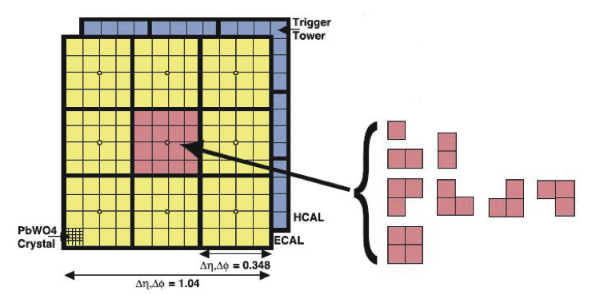
\includegraphics[scale = 0.7]{/home/anter/Desktop/Thesis/Figures/Jet_trigger.png}\\
\vspace*{4mm}
\caption[Muon]{Illustration of the available tower granularity for the L1 jet finding algorithm in the
central region, |η|<3 (left). The jet trigger uses a 3×3 calorimeter region sliding window technique which spans the full(η,φ)coverage of the calorimeter. The active tower patterns allowed for L1τjet candidates are shown on the right Work flow of the L1 trigger system \cite{Chatrchyan:2008aa}.}
\label{fig:Jettrigger}
\end{center}
\end{figure}
\end{comment}
Triggers based on jet and missing transverse energy (\ETmiss) triggers are important for search for new physics whereas the single-jet triggers are mainly designed to study quantum chromodynamics (QCD). In this thesis, the single-jet triggers are used to select the events for analysis. At L1, they use mainly information from the calorimeter by looking for an energy cluster and a high energy deposit. The sums of transverse energy from ECAL and HCAL are computed in 4 $\times$ 4 trigger towers, except in the HF region where this quantity is measured in the whole trigger tower itself. If this deposit is greater than a certain threshold, the event is selected at L1 and it is passed to the HLT. Jets are reconstructed in the HLT using the anti-\kt jet clustering algorithm. The inputs for the jet algorithm are either calorimeter towers giving ``CaloJet'' objects, or the reconstructed particle flow objects giving ``PFJet'' objects. The processing time of reconstruction algorithm is high and hence the jet trigger paths are divided into multiple selection steps. At first, jets are reconstructed from calorimeter towers. Only for events in which at least one calorimeter jet passes a certain \pt threshold, the particle flow algorithm is run and the jets are clustered again from the particle flow candidates. In 2012, most of the jet trigger paths use PFJets as their inputs. The rate of jet events is quite high, so PFJet trigger paths have a pre-selection based on CaloJets. The matching between CaloJets and PFJets is required in single PFJet paths. Due to the flexibility of the HLT, it is possible to apply the jet energy corrections during the HLT selection.

\subsubsection{Data Acquisition System}
As the L1 trigger accepts events at a rate of 100 kHz, the Data Acquisition (DAQ) system has to process the events at the same speed. It reads out the data of all detector sub-components and assembles the complete events, see Fig.~\ref{fig:DAQ}. The data is subsequently passed to the HLT which further reduces the rates to a few hundred events per second. Finally, the events are merged and saved to a local storage system, from which they are continuously transferred to the Tier-0 computing center at CERN.

\begin{figure}[!h]
\begin{center}
\vspace*{3mm} 
\hspace*{-5mm}
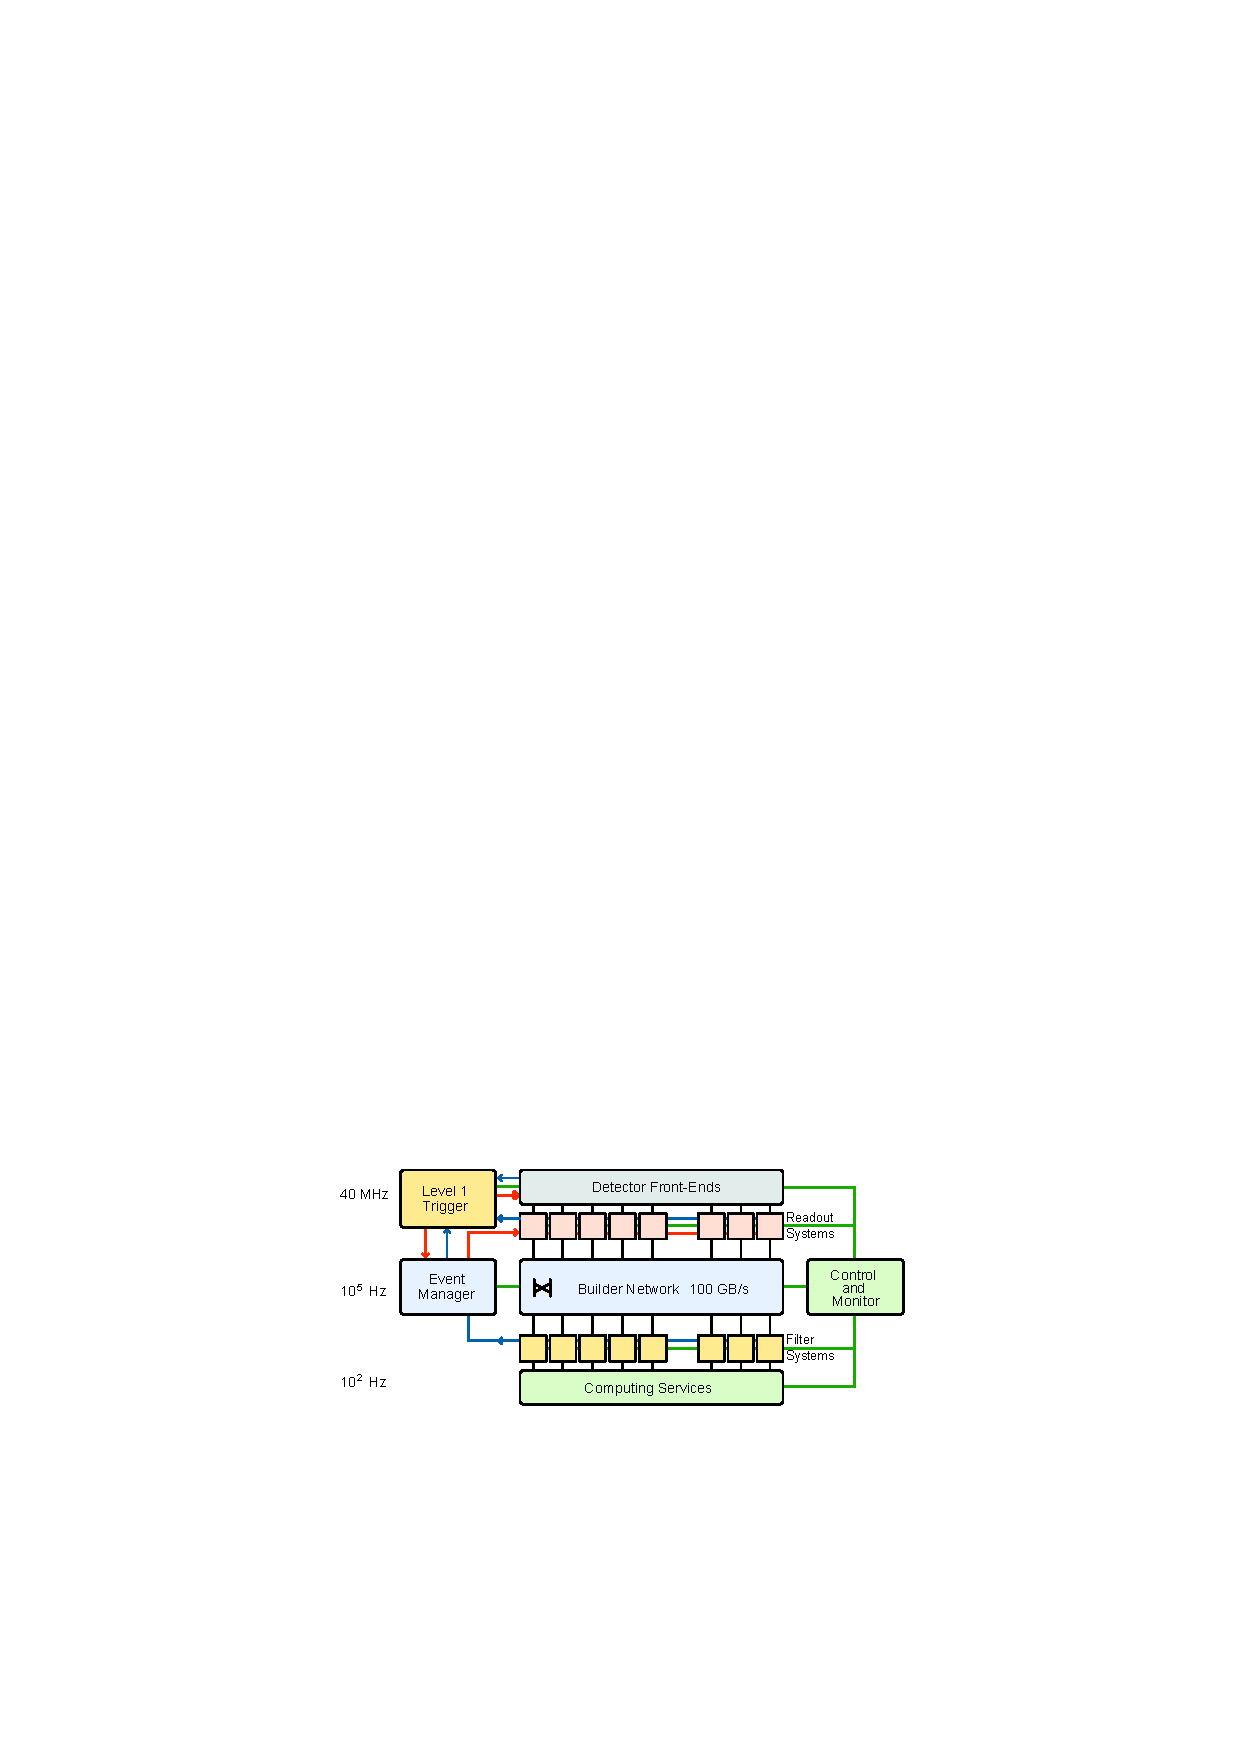
\includegraphics[scale = 1.3]{/home/anter/Desktop/Thesis/Figures/cropped_DAQ.pdf}\\
\vspace*{4mm}
\caption[Architecture of the CMS DAQ system.]{Architecture of the CMS DAQ system. Taken from \cite{Chatrchyan:2008aa}.}
\label{fig:DAQ}
\end{center}
\end{figure}

\subsection{Data Management}
Although the trigger system reduces the collision rate enough to be stored in tape, still there is a huge amount of data need to be analyzed. An efficient computing infrastructure and the software is required for storing and distributing the data. To meet this need, the LHC has a data storage infrastructure called the Worldwide LHC Computing Grid (WLCG) \cite{Bird:2005js}. WLCG provides a hierarchical structure, as shown in Fig.~\ref{fig:Computing}, in a series of four levels or Tiers. Each Tier is made up of several computer centres. All the raw collision data collected by CMS is converted into a format suitable for offline analysis and sorted in the form of data sets at the Tier-0 site at CERN. This processed data is then transferred to Tier-1 centers all over the world where reconstruction algorithms are run. Further reconstructed and simulated data is distributed to Tier-2 sites, where it is available for physics analysis mainly performed on Tier-3 sites. %The powerful Monte Carlo event generators are required to simulate the collision events and these are dicussed in the next chapter.

\begin{figure}[!h]
\begin{center}
\vspace*{3mm} 
\hspace*{-5mm}
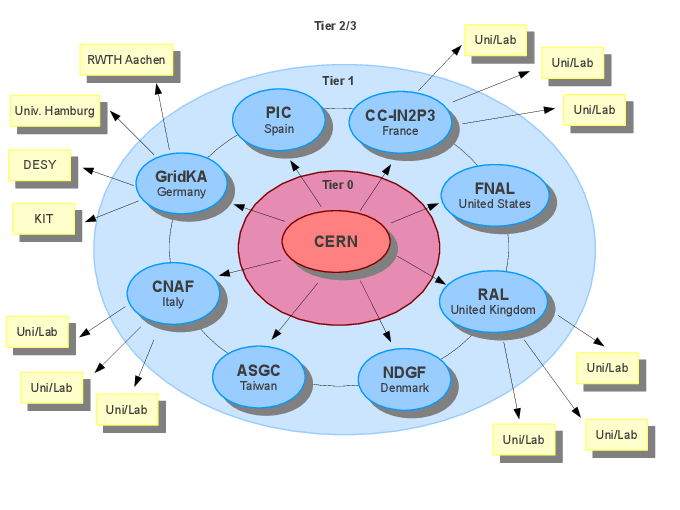
\includegraphics[scale = 0.95]{/home/anter/Desktop/Thesis/Figures/Computing.png}\\
\vspace*{4mm}
\caption[Schematic overview of the CMS computing grid.]{Schematic overview of the CMS computing grid. All data collected by CMS is stored at the Tier-0 site at CERN which is then transferred to Tier-1 centers all over the world. Further reconstructed and simulated data is distributed to Tier-2 sites, where it is available for physics analysis mainly performed on Tier-3 sites. Taken from \cite{Bird:2005js}.}
\label{fig:Computing}
\end{center}
\end{figure}
\cleardoublepage
